
\chapter{Implementación}\label{cap:implementacion}

\section{Herramientas y software utilizado}

En esta sección hablo de las herramientas y software utilizado en el proyecto. \newline

El desarrollo de la aplicación web se ha hecho en el lenguaje de programación \textit{Python}, en su versión \textit{3.9}. Se ha usado \textit{Django} como framework de la APP. \newline

El entorno de desarrollo o IDE utilizado ha sido \textit{PyCharm}. Con la cuenta institucional de la universidad tenemos un año gratis de \textit{PyCharm} \textit{Professional}. Esta licencia nos aporta ventajas a la hora de desarrollar en \textit{Python}, como el \textit{debugger} remoto, útil para debugar código \textit{Python} mapeado a directorios dentro de contenedores \textit{Docker}, por ejemplo. \newline

Se ha usado \textit{git} como controlador de versiones y concretamente, he usado la app \textit{GitHub Desktop}. Esta aplicación aporta una interfaz gráfica de \textit{GitHub} para facilitar la subida de commits, archivos al stage, ramas, etc. También permite ver las diferencias de un mismo archivo en distintas ramas o crear \textit{Pull Requests}, entre otras cosas. \newline

La plataforma de trading usada para el desarrollo ha sido \textit{MetaTrader5}, como ya se ha especificado en secciones anteriores del documento. Se ha elegido esta plataforma ya que dispone de una integración o librería en \textit{Python}. A través de esta librería podemos obtener datos de mercados financieros y conectarnos a cualquiera de los brokers que trabajan con \textit{MetaTrader5} (véase punto \ref{brokers}). Como mencionan en su página, el paquete \textit{MetaTrader} para \textit{Python} está diseñado para obtención de datos directamente del terminal de \textit{MetaTrader5}. Dichos datos pueden ser usados para cálculos estadísticos y aprendizaje automático. Además, la librería permite mandar órdenes de compra y venta directamente desde el propio código. \newline

Debido a que esta dependencia sólo está disponible para Windows, \textit{Windows 10 Home} ha sido el sistema operativo elegido para el desarrollo del proyecto. Para usad Django en Windows, es necesario instalar \textit{Visual Studio C++} en su versión \textit{14.0} o superior. \newline

Para la interfaz gráfica del proyecto se utiliza el lenguaje de marcas \textit{HTML} y para aplicar estilo en estas vistas se utiliza \textit{CSS}. Utilizo también \textit{Javascript} para añadir scripts y lógica adicional en las vistas.\newline

Finalmente, para gestión de bases de datos, se utiliza \textit{SQLite}, en su versión \textit{3}. Este es el sistema gestor de bases de datos de Django por defecto.\newline

Para el desarrollo de este documento, se utiliza \textit{LaTex} y más concretamente, el IDE \textit{TexStudio}. \newline

\begin{figure}[!tbp]
	\begin{subfigure}[b]{0.10\textwidth}
		
\includegraphics[width=\textwidth, height=\textwidth]{imagenes/software_usado/icono_python.png}
		\caption{Python}
	\end{subfigure}
	\hfill
	\begin{subfigure}[b]{0.1\textwidth}
		
\includegraphics[width=\textwidth, height=\textwidth]{imagenes/software_usado/icono_django.png}
		\caption{Django}
	\end{subfigure}
	\hfill
	\begin{subfigure}[b]{0.1\textwidth}
		
\includegraphics[width=\textwidth, height=\textwidth]{imagenes/software_usado/pycharm_logo.png}
		\caption{PyCharm}
	\end{subfigure}
	\newline
	\begin{subfigure}[b]{0.10\textwidth}
		
\includegraphics[width=\textwidth, height=\textwidth]{imagenes/software_usado/icono_html.png}
		\caption{HTML}
	\end{subfigure}
	\hfill
	\begin{subfigure}[b]{0.1\textwidth}
		
\includegraphics[width=\textwidth, height=\textwidth]{imagenes/software_usado/icono_css.png}
		\caption{CSS}
	\end{subfigure}
	\hfill
	\begin{subfigure}[b]{0.1\textwidth}
		
\includegraphics[width=\textwidth, height=\textwidth]{imagenes/software_usado/icono_javascript.png}
		\caption{JavaScript}
	\end{subfigure}
\newline
\begin{subfigure}[b]{0.10\textwidth}
	
\includegraphics[width=\textwidth, height=\textwidth]{imagenes/software_usado/icono_windows.png}
	\caption{Windows}
\end{subfigure}
\hfill
\begin{subfigure}[b]{0.1\textwidth}
	
\includegraphics[width=\textwidth, height=\textwidth]{imagenes/software_usado/icono_visual_studio.png}
	\caption{VSCode}
\end{subfigure}
\hfill
\begin{subfigure}[b]{0.1\textwidth}
	
\includegraphics[width=\textwidth, height=\textwidth]{imagenes/software_usado/icono_sqlite.png}
	\caption{SQLite}
\end{subfigure}
\newline
\begin{subfigure}[b]{0.1\textwidth}
	
\includegraphics[width=\textwidth, height=\textwidth]{imagenes/software_usado/icono_github_desktop.png}
	\caption{GitHub Desktop}
\end{subfigure}
\hfill
\begin{subfigure}[b]{0.1\textwidth}
	
\includegraphics[width=\textwidth, height=\textwidth]{imagenes/software_usado/icono_texstudio.png}
	\caption{TexStudio}
\end{subfigure}
\hfill
\begin{subfigure}[b]{0.1\textwidth}
	
\includegraphics[width=\textwidth, height=\textwidth]{imagenes/software_usado/icono_metatrader5.png}
	\caption{MetaTrader5}
\end{subfigure}

	\caption{Logos de las principales herramientas usadas en el proyecto.}
\end{figure}

\section{Metodología de trabajo}

El trabajo se desarrolla siguiendo la metodología de desarrollo ágil \textit{scrum}. Este tipo de planificación hace que las distintas tareas que se desarrollan se puntúen siguiendo un modelo de puntuación basado en dificultad. En dicha planificación, las tareas se reparten en \textit{sprints} o iteraciones. Una iteración puede durar entre 2 y 4 semanas. En el caso de mi proyecto, los sprints han sido períodos variables de entre 2 y 3 semanas. El uso de scrum y cada uno de los sprints en los que divido el proyecto se mencionan más detalladamente en el punto \ref{fases} de esta memoria.\newline

Como controlador de versiones hemos utilizado \textit{git}, y la plataforma \textit{GitHub}.
Para la correcta y eficiente realización del proyecto, ha sido esencial \textit{GitHub}, ya que es una plataforma que ayuda a llevar una buena estructuración del trabajo gracias a cosas como las \textit{issues}, los \textit{pull request} y sus respectivas revisiones; el trabajo con ramas o \textit{branches}, etc. \newline

	El proyecto se ha desarrollado en su totalidad en el repositorio de \textit{GitHub}: \color{blue} \href{https://github.com/mcarmona99/TFG/}{https://github.com/mcarmona99/TFG/} \color{black}
	
\subsection{Issues y Pull Requests}

Cada tarea se ha representado mediante \textit{issues}. Una \textit{issue} es una descripción de la tarea donde se pueden incluir a miembros del grupo que estén trabajando en la misma, errores específicos de la tarea, versiones del proyecto donde hay que realizarla o aparece el error, etc. \newline

Cada issue suele ser referenciada por un \textit{pull request}. Los pull request son otro tipo de herramienta que sirven para incluir el código realizado en la tarea referenciada al proyecto en producción. Los \textit{PR} explican el proceso y/o el código que se ha introducido para arreglar o implementar la tarea que se pedía. La tarea puede ser arreglar un bug, implementar nuevas funcionalidades, etc. Cada PR debe ser revisado por otro miembro del equipo antes de ser aprobado. En el PR también podemos encontrar información útil como la rama de desarrollo que se estaba usando o los commits realizados en la misma.
\newline

En el caso de este proyecto, el seguimiento y revisión de Issues y PRs ha sido hecho por el mismo desarrollador, debido a que es un trabajo de una sola persona.\newline

En la figura \ref{issue} y \ref{pr} se pueden ver un ejemplo de \textit{Issue} y su \textit{Pull Request}, respectivamente.

\begin{figure}[h]
	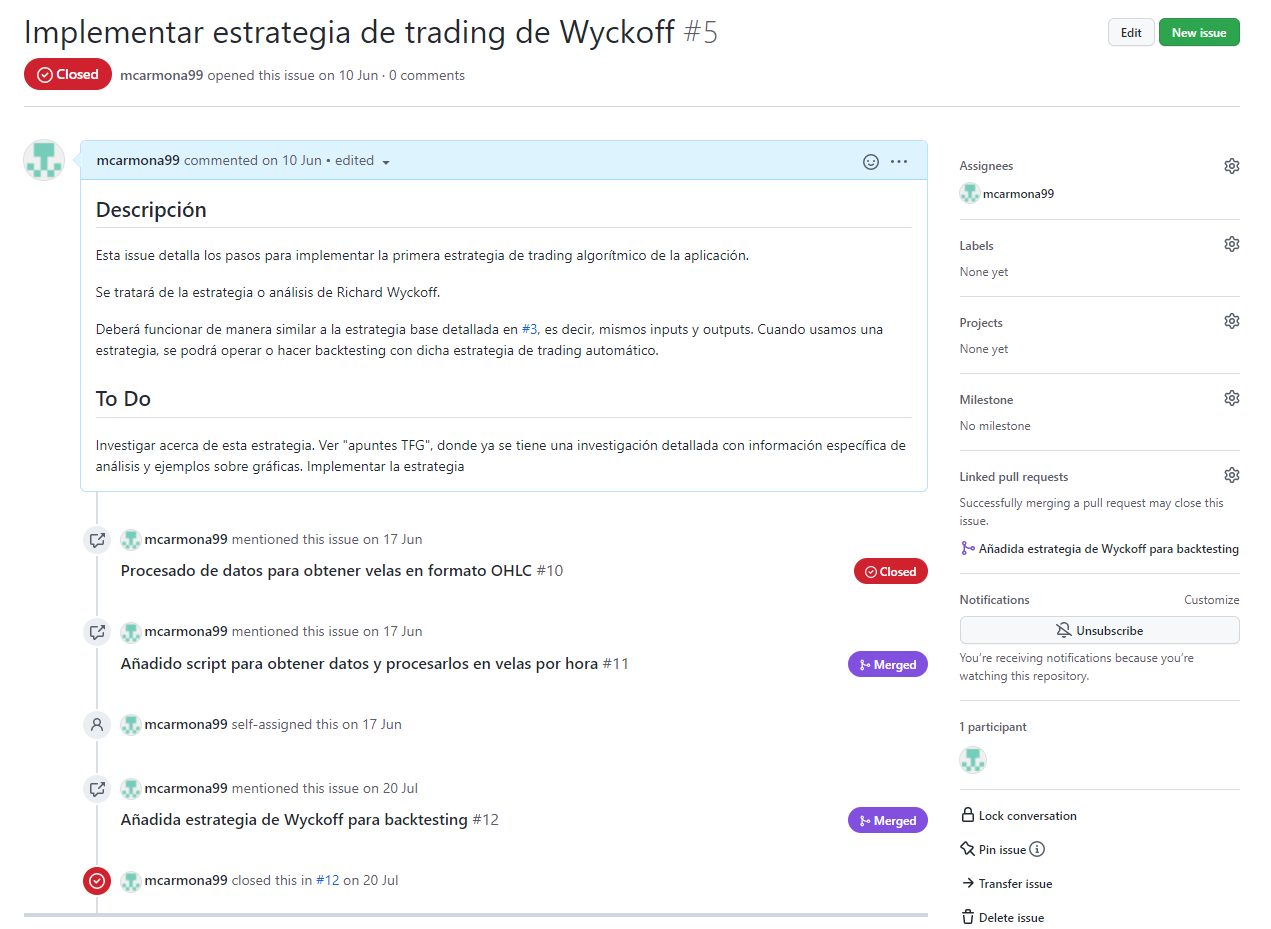
\includegraphics[width=1.2\textwidth]{imagenes/issue_pr/issue.png}
	\caption{\textit{Issue} número 5, implementación de la estrategia de Wyckoff} \label{issue}
\end{figure}

\begin{figure}[h]
	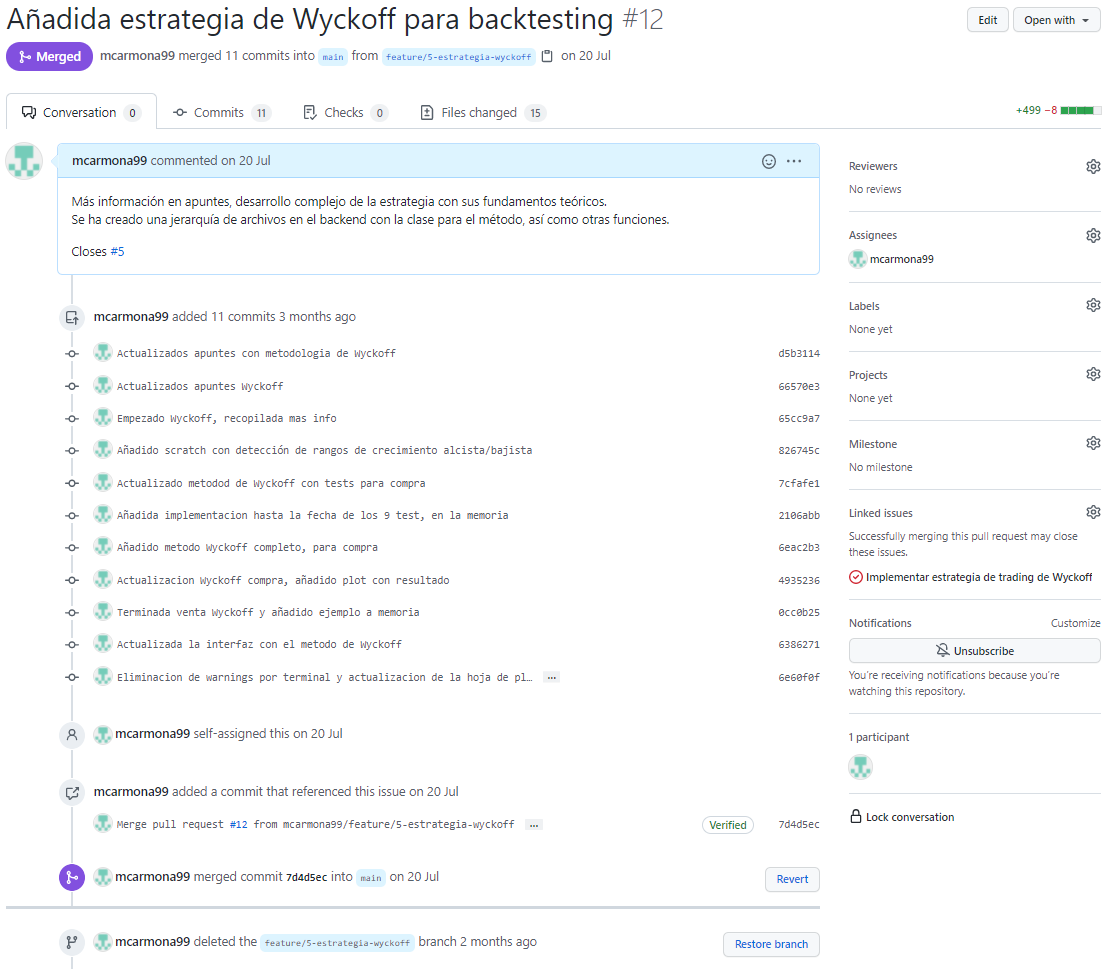
\includegraphics[width=1.2\textwidth]{imagenes/issue_pr/pr.png}
	\caption{\textit{Pull Request} referente a la issue \ref{issue}} \label{pr}
\end{figure}

\subsection{Paralelismo usando GitFlow}

\textit{GitFlow} es un flujo de trabajo basado en \textit{git} que brinda un mayor control y organización en el proceso de integración continua.\newline

El flujo de trabajo con GitFlow se basa principalmente en dos ramas; la rama \textit{develop} y la rama \textit{master}. La rama develop es aquella rama donde convergen las ramas de desarrollo. La rama master, en cambio, es la rama principal y estable (develop también es considerada estable). Esto puede variar en los desarrollos. En mi caso, \textit{main} es la rama que haría de \textit{develop} y a la que se incluyen los desarrollos.\newline

Los nuevos desarrollos parten de la rama develop y se mergean en ella misma una vez se han revisado. Dichos nuevos desarrollos son realizados en ramas que tienen nomenclaturas similares a:\newline

\begin{itemize}
	\item \textbf{feature/\#issue-descripcion-desarrollo}: rama que introduce una nueva funcionalidad.
	\item \textbf{fix/\#issue-descripcion-arreglo}: rama que introduce un fix a un bug o error conocido. En ocasiones tenemos hotfix o bugfix en lugar de fix.
	\item \textbf{support/\#issue-descripcion}: para soporte de pago o soporte a usuarios.
	\item \textbf{release/\#issue-descripcion}: para ramas de release.
\end{itemize}	

Cuando estos desarrollos han terminado, como hemos dicho anteriormente, sus ramas correspondientes son mergeadas a develop, por medio de un Pull Request. Lo normal es que cada PR esté asignado a una issue y a una rama.
\newline

Esto no ha sido de mucha utilidad en el caso de este proyecto, ya que no ha sido un trabajo en el grupo con lo que las ventajas de \textit{GitFlow} no se han visto en gran medida. \newline

\section{Fases del desarrollo} \label{fases}

En esta sección se detallan los \textit{sprints} seguidos en el desarrollo del proyecto. Como se ha mencionado en el punto anterior, los sprints son iteraciones del desarrollo del producto que incluyen un número de tareas a realizar. Los sprints son vitales para llevar a cabo un seguimiento del trabajo hecho hasta el momento. \newline

En el caso de mi trabajo, las fases de desarrollo se han realizado en 6 sprints o iteraciones. Cada uno de estos sprints han durado un período de entre 2 y 4 semanas. \newline

Para llevar una correcta planificación del trabajo, los sprints e issues o tareas incluidas en cada uno de ellos han sido añadidos a una tabla u hoja de planificación. Los cambios de sprints coinciden con las entrevistas realizadas con el tutor del proyecto, ya que han servido para entrega de tareas realizadas y comentarios; e inicio de período con nuevas tareas.\newline

\subsection{Guía de puntuación scrum y prioridades}

En la hoja de planificación he incluido una guía de puntuación de scrum que intenta añadir una equivalencia en horas a cada una de las puntuaciones disponibles en scrum para issues. \textbf{En la teoría de scrum esto se debe evitar}, ya que la puntuación de scrum es una medida de esfuerzo en el trabajo, y no de tiempo invertido. A pesar de esto, he decidido crear la equivalencia para tener un seguimiento más preciso de lo que se ha tardado en cada issue o tarea. \newline 

En la figura \ref{guia_puntos} se encuentra esta guía, cuando menciono días, supongo la equivalencia de un día igual a una jornada de trabajo completa, es decir, 8 horas.\newline

\begin{figure}
	\begin{center}
	\begin{tabular}{| c | c |}
		\hline
		\multicolumn{2}{ |c| }{Guía puntuación SCRUM} \\ \hline
		Puntos & Equivalencia \\ \hline
		1 & 3 horas \\ \hline
		2 & 6 horas \\ \hline
		3 & 1 día \\  \hline
		5 & 2 días \\ \hline
		8 & 3 días \\ \hline
		13 & 5 días \\ \hline
		20 & 7 días \\ \hline
	
	\end{tabular}
	\caption{Guía de puntuación scrum}  \label{guia_puntos}
	\end{center}
\end{figure}

Además de esta guía, en la hoja he añadido una guía sobre las prioridades que he asignado a cada issue dentro de un mismo sprint. Estas prioridades indican lo más o menos importante o vital que se considera una issue con respecto al desarrollo del proyecto. \newline

Los niveles son, en orden de menor a mayor prioridad: \newline
\begin{itemize}
	\item \textbf{Muy baja}: funcionalidad que suele ser de diseño de la interfaz y que incluye cambios al funcionamiento principal de la aplicación. Menor prioridad.
	\item \textbf{Baja}: funcionalidades de diseño de la interfaz que sí que afectan aunque en poca medida al uso de la APP por parte del usuario final.
	\item \textbf{Media}: funcionalidad que necesita ser desarrollada pero con menor prioridad que otras que forman parte del desarrollo principal de la APP.
	\item \textbf{Alta}: funcionalidades pertenecientes al desarrollo principal de la aplicación.
	\item \textbf{Muy alta}: funcionalidades cuyo desarrollo es vital o \textit{stopper} para otros desarrollos. Mayor prioridad posible.
\end{itemize}


\subsection{Fase previa a los sprints de desarrollo}

En este apartado hablaré a grandes rasgos de algunas de las pruebas y desarrollos que hice previos a los inicios de lo que es el desarrollo principal de la APP y por tanto, de los sprints. \newline

En primer lugar, se invirtió tiempo desarrollando algunos scripts de Python para conectar con interfaces externas de Trading. En este punto se investigó sobre Binance y su librería para Python \textit{python-binance}. \newline

Fue en esta etapa cuando empecé a usar la integración de MetaTrader5 en Python, siguiendo los tutoriales oficiales de la web: \href{https://www.mql5.com/es/docs/integration/python_metatrader5}{Módulo MetaTrader para la integración con Python
}. Además de esto, estuye leyendo sobre el lenguaje de \textit{MQL5}, que es el proporcionado por MetaTrader y su integración por Python. Este proceso es más complejo y busca conectar procesos en sockets de red, para conectar una aplicación con el terminal de MetaTrader. Debido a la facilidad de uso, me decanté por la primera opción, usar la librería de \textit{MetaTrader} en Python. \newline

En segundo lugar, se investigó sobre Django. En este período desarrollé los tutoriales ofrecidos en la página oficial de Django y diferencié los conceptos de proyecto y aplicación, migraciones, estructura de la base de datos, etc. \newline

En una tercera fase previa al desarrollo, estuve investigando cómo obtener datos históricos de los distintos mercados financieros soportados por MetaTrader, tal y como se acordó con el tutor del proyecto. Estos datos históricos serían los inputs de cada uno de los algoritmos para trading desarrollados. Los datos se sacaron con script que conectaban al terminal de MT5.\newline

En esta investigación conseguí sacar 1 o 2 años de datos de cada uno de los mercados de MetaTrader5, dependiendo de la disponibilidad. En total, conseguí obtener datos de 179 mercados. MetaTrader5 dispone de 570 mercados en total, pero la librería de Python solo soporta datos de esos 179 mercados. \textbf{Problema presentado}: a pesar de que los datos en sí no consumían una gran cantidad de memoria, MetaTrader5 cacheaba todos los mercados y los monitorizaba al haber cogido datos de los mismos. Es por esto que estuve teniendo problemas de capacidad de disco. A raíz de esto, se decidió hacer un cambio en el planteamiento y \textbf{optamos por tomar el máximo numero de años de datos posibles de 5 mercados financieros de distinta naturaleza disponibles en MT5}. Esto dio lugar a tomar 1 mercado de Forex, 2 mercados de metales; y 2 mercados de energías. Dichos mercados serían el \textit{Euro vs Dólar}, \textit{Euro vs Plata}, \textit{Dólar vs Oro}, \textit{Petróleo Brent vs Dólar} y \textit{Gas Natural vs Dólar}. \newline

Los datos obtenidos se pueden observar en la figura \ref{datos_obtenidos}. Como se puede ver, se sacan 10 años de \textit{EURUSD} (euro-dólar); y 5 años de \textit{XBRUSD} (brent-dólar), \textit{XNGUSD} (gas natural-dólar), \textit{XAGEUR} (plata-euro) y \textit{XAUUSD} (oro-dólar). Estos datos incluyen precios y otro tipo de información otorgado por MT5. \newline

\begin{figure}[h]
	\centering
	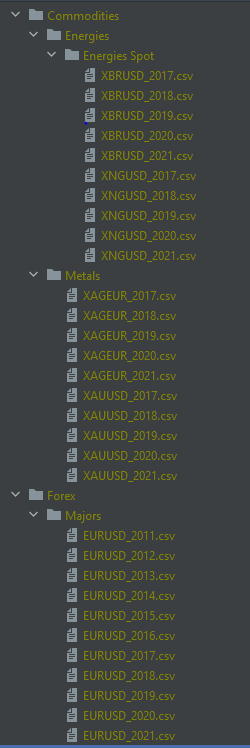
\includegraphics[width=0.35\textwidth]{imagenes/datos_obtenidos.png}
	\caption{Datos de mercados obtenidos en las fases previas al desarrollo} \label{datos_obtenidos}
\end{figure}

\subsection{Sprint 1: 8 junio - 22 junio. Interfaces y modelos básicos}

En esta sección hablaré de las issues y demás tareas realizadas en el sprint 1. Este sprint comprende desde el 8 de junio hasta el 22 de junio de 2021. \newline

En este sprint se realizaron las siguientes cuatro issues: \color{blue}\href{https://github.com/mcarmona99/TFG/issues/1}{\#1}, \href{https://github.com/mcarmona99/TFG/issues/3}{\#3} \href{https://github.com/mcarmona99/TFG/issues/4}{\#4}, \href{https://github.com/mcarmona99/TFG/issues/7}{\#7} \color{black}y\color{blue} \href{https://github.com/mcarmona99/TFG/issues/10}{\#10}\color{black}. \newline

\subsubsection{Issue 1: Creación de la interfaz principal de la APP}

Esta issue es la inicial y fue catalogada con prioridad Muy alta. Como se indica en la guía de prioridades del apartado anterior, este nivel equivale a issues vitales o stoppers. En este caso, la issue detalla la primera tarea. Esta tarea es la creación de la interfaz principal de la aplicación siguiendo el diseño propuesto en la memoria del proyecto. \newline

El diseño que menciono es aquel comentado en el punto \ref{primer_diseño}, donde se expone el primer diseño de la interfaz. \newline

La issue no incluye investigaciones sobre Django ya que eso se realiza en lo que hemos llamado como\textit{ Fases previas al desarrollo} y que se puede encontrar en el punto de la planificación y en el diagrama de Gantt del proyecto. En otras palabras, en esta issue se monta el esquema de la interfaz de la aplicación web en Django conociendo ya el software y cómo proseguir. \newline

En el \color{blue}\href{https://github.com/mcarmona99/TFG/pull/6}{pull request} \color{black}conectado a esta issue encontramos los cambios añadidos y la interfaz creada. En dicho PR se comenzó el proyecto de \textit{Django} y se creó la primera APP llamada \textit{Interface}. Se desarrolló por tanto la interfaz o menú principal en una vista que se obtiene al pedir la request a \textit{/}, es decir, primera página de la web. Las vistas se han creado usando \textit{HTML} y estilos de \textit{CSS}. Se crean también los botones del diseño sin funcionalidad. \newline

\subsubsection{Issue 7: Creación de la interfaz para elección de estrategias}

En esta issue se pide crear la interfaz y modelos básicos para poder ver desde el botón \textit{Estrategias de Trading} cada una de las estrategias y poder elegirlas, creando la lógica de modelos que se necesite para asignar la estrategia a la sesión actual. \newline

Para la resolución de esta issue se crea una interfaz a la que se accede con el botón \textit{Estrategias de trading}. Para ello se ha necesitado un modelo llamado \textit{Sesion}. La clase \textit{Sesion} solo tendrá en primer lugar 1 instancia y será equivalente a la sesión actual (hasta que se implemente la gestión de usuarios, cada usuario tendría la misma sesión). La sesión contiene la estrategia de trading seleccionada. \newline

Además se crea otro modelo llamado \textit{AlgoritmoTrading}, que representará cada uno de los algoritmos a elegir. \newline

Se crea la relación: \newline

\textit{Sesion --- tiene $\rightarrow$ AlgoritmoTrading} \newline

Estos modelos se pueden ver en el diagrama de clases del proyecto.\newline

Esta issue y por tanto la creación de la lógica de modelos mencionada es completada con el PR \href{https://github.com/mcarmona99/TFG/pull/8}{\#8}.\newline


\subsubsection{Issues 4 y 3: Backtesting con estrategia y estrategia de trading algorítmico base}

En la issue 4 se debe implementar la funcionalidad de backtesting. Esta funcionalidad se explica en el requisito funcional número 5. \newline

Para esta issue era necesario el desarrollo previo de un modelo básico para realizar testing, con lo que esta issue se fusiona con la issue \href{https://github.com/mcarmona99/TFG/issues/4}{\#3}. La estrategia propuesta como base será la estrategia de medias móviles. La issue se cierra con el PR \color{blue}\href{https://github.com/mcarmona99/TFG/pull/9}{\#9}\color{black}. \newline

\textbf{En primer lugar, para la implementación de la estrategia de medias móviles, issue \#3:}\newline

Podemos empezar comentando el por qué usar una media móvil. Las medias móviles nos ayudan a eliminar el ruido en un gráfico de precios. Dichas medias pueden funcionar como soportes o resistencias (véase contexto teórico), es decir, el precio debería de ir por encima. Esto significa que las medias se comportarían como suelos, si el precio las pasa, debería de seguir bajando.\newline

Generalmente, si el precio está por encima de una media móvil, el precio tenderá a caer; y si está por debajo, tenderá a subir. Esto obviamente no siempre ocurre. Además, el comportamiento dependerá de la ventana que estemos utilizando.\newline

Tipos de media móvil:

\begin{itemize}
	\item SMA (simple moving average). Media móvil simple. Un ejemplo sería una media móvil con ventana de 5 días. Dicho valor calcularía la media en un rango de 5 días.
	\item EMA (exponencial moving average). Media móvil exponencial. Esta media da más peso a los precios más recientes. Usa cálculos más complejos. La EMA reacciona más rápido a los cambios del precio que la SMA debido a los pesos en los cálculos.
\end{itemize}

Las ventanas del moving average son los time frame o marcos de tiempo con los que se genera la media. Una ventana de 100 días lleva una media móvil de 100 días vista. En cuanto a los tamaños de ventana, con ventanas más pequeñas la media reaccionará mucho más rápido a los cambios del precio que una media con mayor ventana. En la figura \ref{medias_moviles} podemos ver una ventana de 100 días (azul claro) contra una de 30 días (azul oscuro).\newline

\begin{figure}[h]
	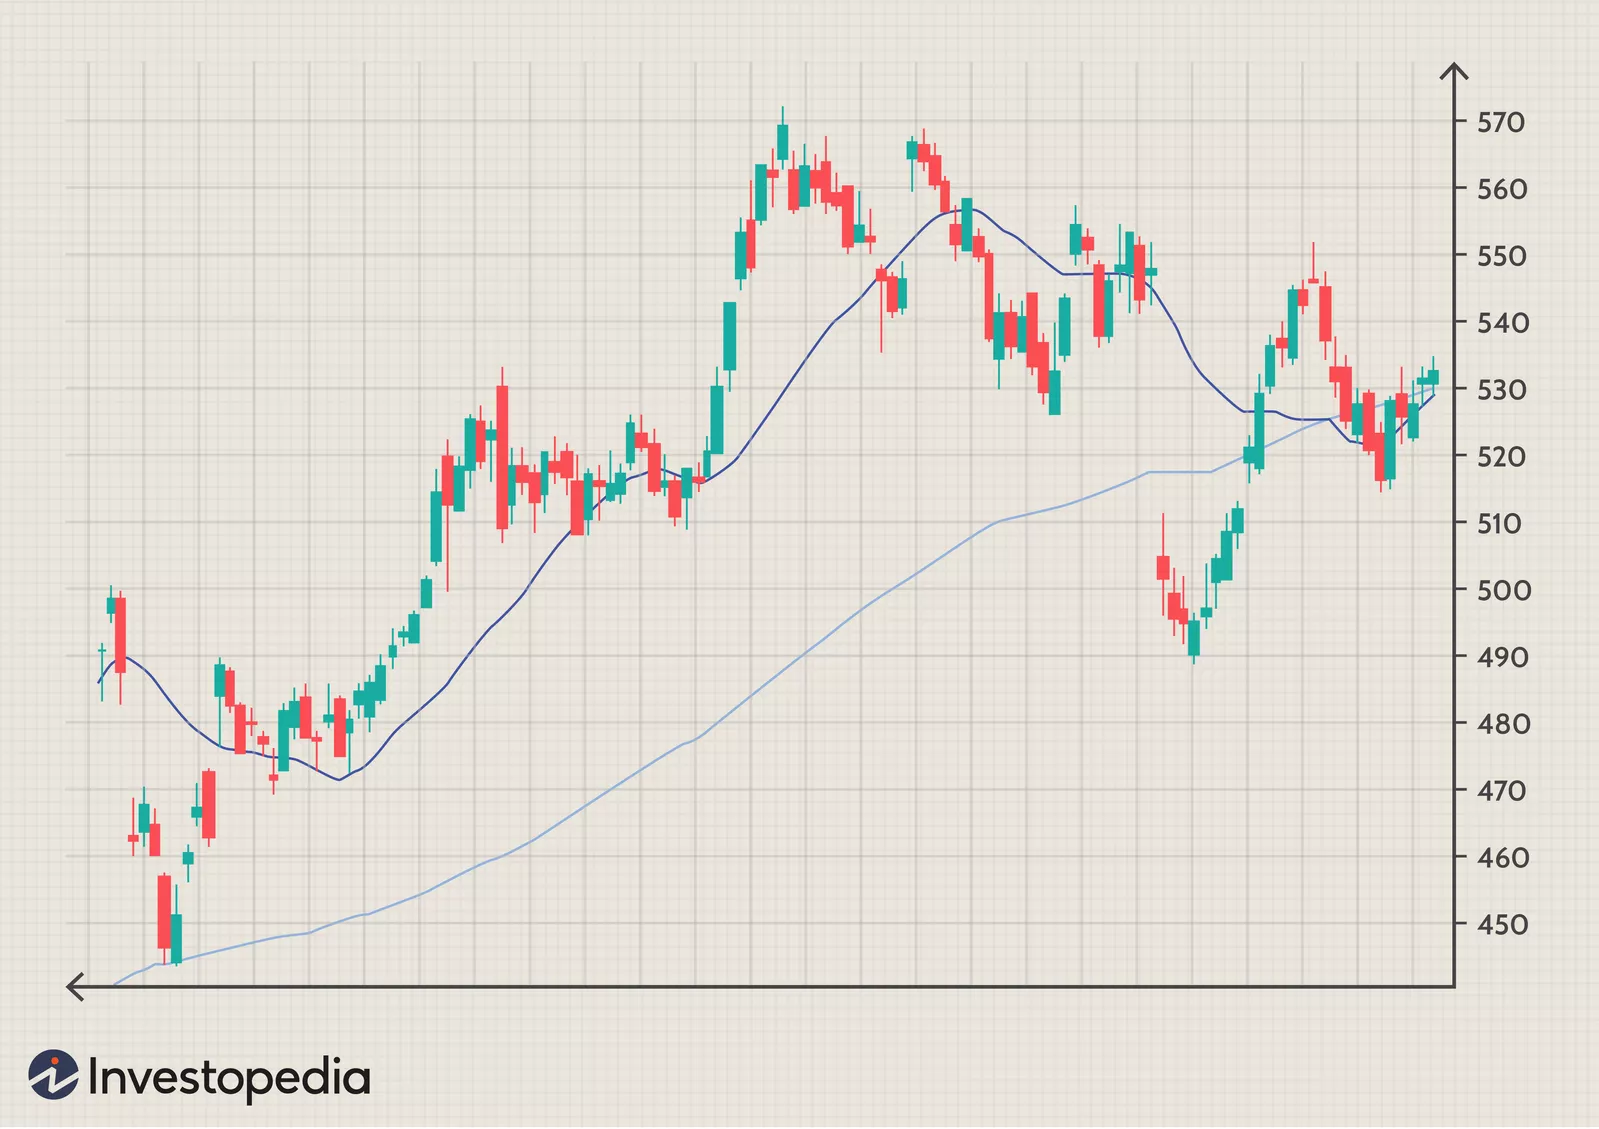
\includegraphics[width=1\textwidth]{imagenes/medias_moviles.png}
	\caption{Media móvil con ventana de 100 días (azul claro) contra ventana de 30 días (azul oscuro). Fuente: \href{https://www.investopedia.com/}{investopedia.com/}} \label{medias_moviles}
\end{figure}

En teoría, las ventanas más grandes benefician más a los traders que operan a largo plazo y las medias con ventanas más pequeñas ayudan más a los de corto plazo.\newline

A la hora del desarrrollo del modelo, se ha tenido en cuenta las señales de compra o venta marcadas por dos medias móviles. Cuando el precio cruza por encima o por debajo de la media móvil señaliza un cambio potencial de tendencia. Al usar dos medias SMA, una con una ventana más grande y otra más pequeña, tenemos el siguiente comportamiento: 

\begin{itemize}
	\item Cuando la MA a corto plazo supera a la de largo plazo $\rightarrow$ señal de compra (golden cross)
	\item Cuando la MA a largo plazo supera a la de corto plazo $\rightarrow$ señal de venta (dead/death cross)
\end{itemize}

\textbf{Finalmente, para la implementación del backtesting con estrategia, issue \#4:}\newline

Añado un atributo al modelo \textit{Sesion} llamado \textit{logued\_MT5} para gestión de botones, ver qué botones disponibles y cuáles no en la interfaz. Por ahora será por defecto \textit{True} para la sesión, hasta que se implemente el login y logout en MT5. \newline

Creo la interfaz inicial para realizar backtesting. \newline

Para operar, creo el modelo \textit{Mercado}, que representa la divisa/mercado financiero en el que se opera, tendrá un nombre y una función para obtener el gráfico (referencia a issue de ver datos de mercado entre rango, aún no realizada). \newline

Creo objetos para el nuevo modelo Mercado, cada uno de ellos referentes a los 5 mercados en los que estamos trabajando.\newline

\begin{figure}[!h]
\begin{lstlisting}
>>> from Interface.models import Mercado
>>> m = Mercado(nombre='XBRUSD')
>>> m.save()
>>> m2=Mercado(nombre='XNGUSD')
>>> m2.save()
>>> m3=Mercado(nombre='XAGEUR')
>>> m3.save()
>>> m4=Mercado(nombre='XAUUSD')
>>> m4.save()
>>> m5=Mercado(nombre='EURUSD')
>>> m5.save()
\end{lstlisting}
\caption{Creación de objetos para el modelo \textit{Mercado}}
\end{figure}

He editado toda la estructura de carpetas de mi proyecto de Django, para usar códigos comunes a los algoritmos, los algoritmos en sí, y hasta que se implemente la gestión de datos, gestión de datos en local. La estructura mencionada se puede ver en la figura \ref{tree}. \newline

\begin{figure}[!h]

\dirtree{%
	.1 TradingAPP.
	.2 Interface.
	.3 backend.
	.3 migrations.
	.3 static.
	.4 css.
	.4 TradingAPP.
	.5 imagenes.
	.3 strategies.
	.3 templates.
	.4 registration.
	.4 TradingAPP.
	.2 TradingAPP.
} 
\caption{Árbol de directorios del proyecto} \label{tree}
\end{figure}

\subsubsection{Issue 10: Procesado de datos para formato OHLC}

En este apartado se describe la issue 10 y su desarrollo.\newline

Esta issue explica la necesidad de desarrollar un procesado de datos para tener los precios en formato OHLC (Open High Low Close). \newline

En el PR \href{https://github.com/mcarmona99/TFG/pull/11}{\#11} se añaden los cambios necesarios para añadir este preprocesado de datos obtenidos de MT5. Para generar los datasets con velas y las columnas de Open, High, Low y Close, se sigue la siguiente guía en la que lo explica cómo hacerlo con pandas: \href{https://blog.quantinsti.com/tick-tick-ohlc-data-pandas-tutorial/?utm_campaign=News&utm_medium=Community&utm_source=DataCamp.com}{Converting Tick-By-Tick Data To OHLC Data Using Pandas Resample}.\newline


\subsection{Sprint 2: 22 junio - 13 julio. Desarrollo del método de Wyckoff}

En este segundo sprint sólo se realiza una issue. La issue consiste en desarrollar la estrategia de trading de Wyckoff o \textit{método de Wyckoff}. La issue es la número \href{https://github.com/mcarmona99/TFG/issues/5}{\#5}; y es cerrada por el PR \href{https://github.com/mcarmona99/TFG/pull/12}{\#12}.\newline

\subsubsection{Issue 5: Implementación del método de Wyckoff}

Como se ha mencionado antes, esta issue detalla los pasos para implementar la primera estrategia de trading algorítmico de la aplicación. \newline

Se tratará de la estrategia o análisis de \textit{Richard Wyckoff}.\newline

Deberá funcionar de manera similar a la estrategia base detallada en la issue \#3, es decir, mismos inputs y outputs. Cuando usamos una estrategia, se podrá operar o hacer backtesting con dicha estrategia de trading automático. \newline

Para la implementación, nos basaremos en el análisis de Wyckoff, descrito minuciosamente en el punto \ref{wyckoff}.\newline

A partir de la teoría de Wyckoff podemos seguir 8 tests de compra y 8 tests de venta, dependiendo de si estamos en una fase de acumulación o de distribución, respectivamente.\newline

Tests de compra para una acumulación vs Tests de venta para una distribución:\newline

\begin{enumerate}
	\item El objetivo bajista se ha cumplido  vs  El objetivo alcista se ha cumplido
	\item Vemos un PS, SC, AR y STs  vs  Vemos un PSY, BC, STs.
	\item Actividad alcista vs Actividad bajista
	\item Tendencia bajista se ha roto (oferta de tendencia bajista rota)  vs  Tendencia alcista rota (línea de soporte ha sido rota)
	\item Mínimos más altos  vs  Mínimos más bajos
	\item Máximos más altos  vs  Máximos más bajos
	\item La acción del precio es más fuerte que el mercado  vs  La acción es más débil que el mercado
	\item Se crea un suelo o soporte (línea de precios horizontal)  vs  Se crea un techo o resistencia (línea de precios horizontal)
\end{enumerate}

Si estos tests se cumplen, ya sea para compra o para venta, podemos incluir nuestra operación con un punto de parada de beneficios 3 veces superior al de pérdidas. Esto es lo que se conoce como \textit{Take Profit} y \textit{Stop Lose}, respectivamente. En un ejemplo práctico, si metemos una compra cuando una acción cuesta 100 \euro, la operativa de Wyckoff nos dice que el TP estará en 115 \euro y el SL en 95 \euro.\newline

En cuanto a la implementación en sí, comencé buscando una forma de investigar cómo reconocer tendencias dentro de un gráfico. Estuve viendo indicadores de análisis técnico. Finalmente decidí implementar una solución que usa \textit{bandas de Bollinger} para detección de intervalos de crecimiento y decrecimineto dentro del gráfico de precios. En otras palabras, detección de tendencias.\newline

Las bandas de Bollinger son un indicador de volatilidad del mercado y proporcionan información de continuidad de tendencia, periodos de consolidación, periodos de amplia volatilidad y posibles máximos y mínimos del mercado.\newline

Dentro de lo que aportan las bandas de Bollinger, me interesa la detección de tendencia y consolidación de mercados, que viene a ser los periodos de acumulación y distribución. \newline

El inicio de la implementación del algoritmo consiste en dibujar las bandas en un gráfico para ver cómo se ven y su comportamiento. En el gráfico de la figura \ref{bandas_bollinger} se puede observar las bandas (líneas naranja, verde y roja) y el precio (línea azul).\newline

\begin{figure}[h]
	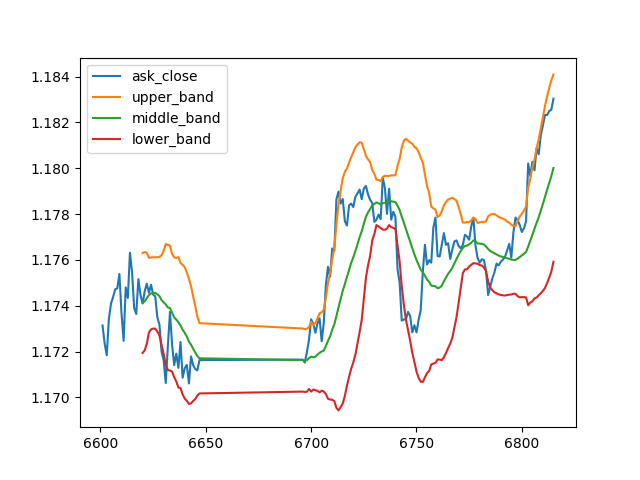
\includegraphics[width=1\textwidth]{imagenes/bandas_bollinger.png}
	\caption{Bandas de Bollinger en un gráfico de precios} \label{bandas_bollinger}
\end{figure}

En el algoritmo de detección de tendencias que desarrollo, lo que hago es hacer un cálculo de la diferencia de bandas en cada punto de la gráfica. En la figura \ref{diferencia_bandas} se puede ver en primer lugar las bandas de Bollinger que hemos visto en la figura anterior como naranja y roja, esta vez de colores azul y naranja, respectivamente. A la derecha de dicha imagen vemos una gráfica que muestra en el eje \textit{y} la diferencia de valores de cada banda de Bollinger en función del valor de \textit{x} (que viene a ser un simple índice).\newline

\begin{figure}[!tbp]
	\begin{subfigure}[b]{0.6\textwidth}
		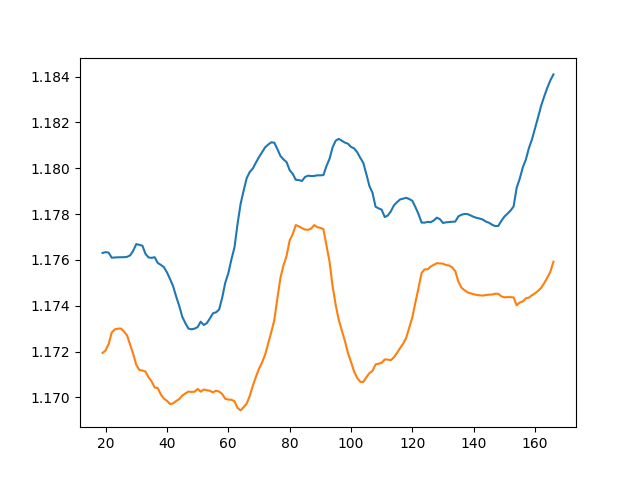
\includegraphics[width=\textwidth]{imagenes/solo_bollinger.png}
		\caption{Bandas de Bollinger}
	\end{subfigure}
	\hfill
	\begin{subfigure}[b]{0.6\textwidth}
		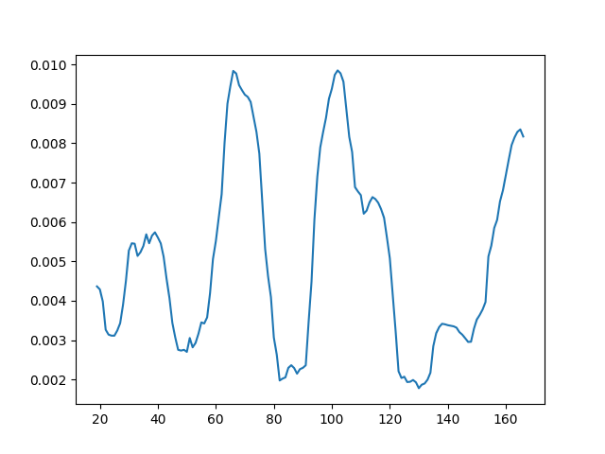
\includegraphics[width=\textwidth]{imagenes/diferencias_bollinger.png}
		\caption{Diferencias de las bandas de Bollinger}
	\end{subfigure}
	
	\caption{Gráficos que representan bandas de Bollinger y diferencia de sus valores} \label{diferencia_bandas}
\end{figure}

Como se puede apreciar, cuando tenemos tendencias, las diferencias de valores en las bandas son mucho más altas que cuando tenemos un período de consolidación: acumulación o distribución.\newline

Aprovechando esto, el algoritmo detectará una tendencia cuando vea un intervalo en el gráfico de precios que las diferencias de las bandas sean consideradas \textbf{anomalías} dentro de los datos. Para que esto sea posible, considero anomalías a aquellos valores que superen la media de valores representados en la gráfica.\newline

Al implementar esto, obtengo los resultados que se pueden ver en la figura \ref{intervalos_detectados}. Los resultados vienen a ser intervalos representados con franjas de color azul en el gráfico. Cabe señalar que estas franjas se detectan en tiempo real, por lo que se han hecho simulando el paso del tiempo y generando dichos intervalos. Como podemos apreciar, vemos que se ha detectado un intervalo o tendencia bajista seguida de una acumulación; una tendencia alcista seguida de una distribución; y una tendencia bajista seguida de otra acumulación. \newline

\begin{figure}[h]
	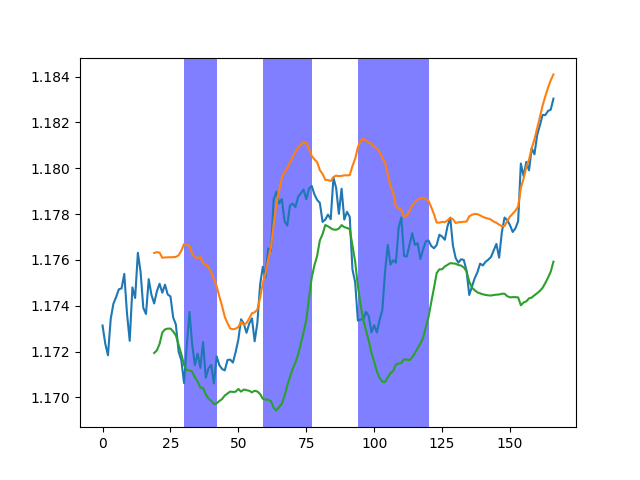
\includegraphics[width=1\textwidth]{imagenes/intervalos_detectados.png}
	\caption{Intervalos detectados con el algoritmo de detección de tendencias} \label{intervalos_detectados}
\end{figure}

\begin{figure}[!tbp]
	\begin{subfigure}[b]{0.6\textwidth}
		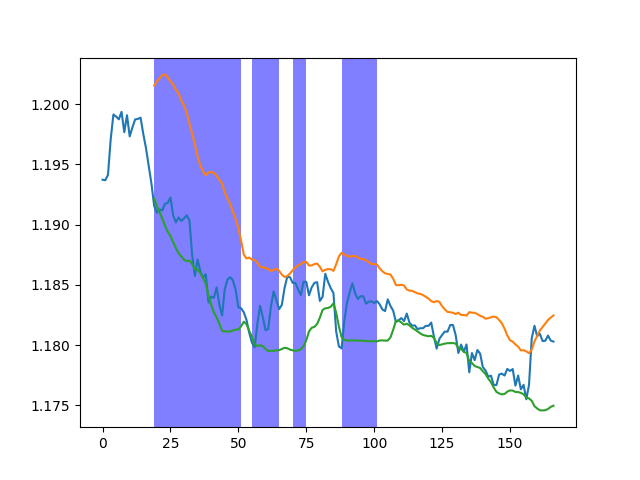
\includegraphics[width=\textwidth]{imagenes/intervalos1.png}
		\caption{Gráfico 1}
	\end{subfigure}
	\hfill
	\begin{subfigure}[b]{0.6\textwidth}
		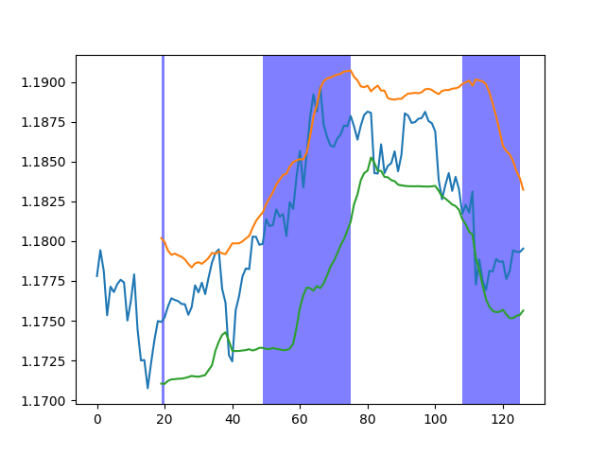
\includegraphics[width=\textwidth]{imagenes/intervalos2.png}
		\caption{Gráfico 2}
	\end{subfigure}
	
	\caption{Otros ejemplos de intervalos detectados con el algoritmo de detección de intervalos}
\end{figure}

Una vez tenemos este algoritmo implementado, procedemos a implementar los 8 tests de compra o venta descritos anteriormente en este mismo apartado. La implementación es la misma tanto para compra como para venta, la única diferencia es cambios de signos y otros cambios menores.\newline

\begin{itemize}
	\item \textbf{Objetivo bajista / alcista cumplido:} detección de intervalos con bandas de Bollinger. Partimos de la base: en periodos bajistas y alcistas, tenemos mucha volatilidad en el precio, cosa que se ve en las bandas (bandas más separadas). En mi implementación del algoritmo para detección de intervalos, compruebo lo siguiente, teniendo datos de precios de la última semana en tiempo real:
	\begin{itemize}
		\item Obtengo un vector de anomalías en cuanto a diferencias de valores de las bandas de Bollinger para cada unidad de tiempo. Una diferencia de valores será una anomalía si su valor es mayor que la media de diferencias.
		\item El vector de anomalías indicará los tiempos en los cuáles tuvimos volatilidad, esto es, indicarán intervalos. 
		\item Para cada anomalía, que es una lista de índices, vemos si el primer valor es mayor o menor que el último, lo que indica alcismo o bajismo.
		\item En el análisis a tiempo real o backtesting, si el vector que estábamos llenando de anomalías se ha cerrado, indicará que hemos terminado un intervalo de crecimiento o decrecimiento.
	\end{itemize}
	\item Vemos un PS, SC, AR y STs / Vemos un PSY, BC, STs:
	\begin{itemize}
		\item No es necesario comprobar que tenemos un PS o PSY, ya que nos indica que está terminando la tendencia. Que la tendencia ha terminado, lo conocemos con lo descrito en el anterior punto, el algoritmo de detección de tendencias con anomalías en las bandas de Bollinger.
		\item SC → el Selling Climax indica que la amplitud del precio y presión de la oferta llegan a su clímax. A efectos prácticos el SC es el mínimo absoluto del intervalo de decrecimiento detectado. Se aplica lo análogo para detectar el BC, buying climax.
		\item AR → el Automatic Rally hace subir los precios fácilmente. El máximo de este rally ayudará a definir el límite superior del siguiente rango de acumulación (mercado lateral). En mi implementación lo tomo como el máximo de los valores que hay a partir del SC hasta que llego al fin del intervalo de decrecimiento detectado. A fin de cuentas, la teoría dice que el AR es justo eso, una subida de precios tras llegar al SC y eso lo reúne también mi algoritmo, aunque puede darse que después del SC no haya máximos muy marcados que puedan indicar un AR. Se aplica lo análogo para detectar el Automatic Reaction.
		\item El ST, secondary test, se produce cuando se supera alguna de las líneas que marcan el rango de acumulación. Estas líneas son determinadas por el SC y el AR. Se determina que un punto es un ST según si está cerca del SC un tanto por ciento, cosa que podemos determinar conociendo el rango de acumulación que sería de tamaño AR - SC. Se aplica lo análogo para detectar los tests en venta.
	\end{itemize}
	\item Tendencia bajista rota: Implementado con una media móvil. Esta tendencia no es lo mismo que el intervalo anterior, que nos indica un bajismo mas “brusco” y directo. Esta tendencia se refiere a la actuación del precio con una perspectiva anterior. Si hemos superado a la media móvil, hemos roto dicha tendencia. Análogo para la venta.
	\item Mínimos más altos: Voy guardando máximos y mínimos y comparándolos en cada iteración. Añado por cada mínimo mas alto, cierto valor al indicador para operar, que será un entero y tras superar un valor, indicará la compra o venta, dependiendo de la fase en la que estemos. Análogo para la venta.
	\item Máximos más altos: Mismo procedimiento que en el punto anterior.
	\item Se crea suelo o soporte: Este suelo o techo lo determina el rango descrito anteriormente cuando he hablado de los STs. Este rango se hace entre AR y el SC. Cuando superamos el mínimo valor del suelo, salimos de la posible compra. Análogo para la venta con techo o resistencia.
\end{itemize}

Una vez descrito esto, compraremos o venderemos si se han cumplido 5 de los anteriores operadores. Cada uno suma de manera distinta al proceso y sus valores se han parametrizado según efecto en el precio. Según hemos comentado en secciones anteriores, el TP debe tener el triple de beneficio que el SL. A efectos prácticos, he reducido la relación a x2 para efectuar más compras en menos tiempo y probar el algoritmo de forma más eficaz. \newline

Una vez implementado el análisis de Wyckoff, este puede ser usado tanto en Backtesting como en tiempo real.\newline

\subsection{Sprint 3: 13 julio - 31 julio. Funcionalidad para login y logout en MT5}

Este tercer sprint se corresponde con el período desde el 13 de julio hasta el 31 de julio. En él se realiza la issue \#2 en la que se pide implementar la funcionalidad de login y logout en MT5.\newline

\subsubsection{Issue 2: Implementar funcionalidad de login y logout en MT5}

En la fase de especificación de requisitos, se definió RF-2.1 como:\newline

RF-2.1. Login en la plataforma de trading. El usuario de la aplicación podrá conectarse con su cuenta de trading, comercial o demo, para poder hacer el uso completo de la APP.\newline

En esta issue (\href{https://github.com/mcarmona99/TFG/issues/2}{\#2}) se debe desarrollar esta funcionalidad de forma que podremos usar la interfaz para conectarnos a MT5. Esta funcionalidad es la que implementa también los botones \textit{Login} y \textit{Logout} del menú principal.\newline

En esta issue se implementan dos funciones en un fichero del directorio backend para identificarse con el bróker usado en MT5 y cerrar sesión, respectivamente. La función de login necesita el usuario, la contraseña y el servidor al que se pretende conectar. Dicho servidor es proporcionado por el bróker.\newline

Esta issue es sencilla puesto que la dependencia de MetaTrader tiene funciones para iniciar sesión en MT5. Sólo ha hecho falta adaptarlo a la APP y generar las interfaces gráficas o vistas. \newline

Esta funcionalidad solo nos permite navegar entre cuentas para las que ya hemos estado identificados en el terminal de MT5, por tanto, para que esto funcione, en el terminal de MT5, es decir, la interfaz gráfica, tenemos que haber estado logueados con cada cuenta previamente. MT5 tiene una base de datos, con lo que la password no será necesaria si tenemos esta opción habilitada en el terminal (guardar datos de conexión, que en MT5 es \textit{guardar los ajustes y datos personales al inicio}).\newline

En la APP, el usuario debe de haberse identificado con antelación en el terminal del host. La opción anteriormente mencionada deberá de estar activada. De esta forma, si el usuario de la APP quiere, puede cambiar de usuario de MT5 dentro de la misma sesión de la APP.\newline

De estas identificaciones previas al terminal de MT5 se encargará el administrador de la aplicación.\newline

Además de estas funciones, se ha creado una función auxiliar para matar el proceso del terminal de MetaTrader5 cuando cerramos sesión en nuestra cuenta. Dicha función busca el proceso de MT5 con el módulo de MetaTrader \textit{wmi} y le aplica un \textit{Terminate()}.\newline

\subsection{Sprint 4: 31 julio - 14 agosto. Visualización de datos de mercados y gestión de usuarios}

En este cuarto sprint se recogen las issues de visualización de datos de mercados financieros, en tiempo real y antiguos (issue \href{https://github.com/mcarmona99/TFG/issues/14}{\#14}); y la issue de gestión de usuarios de la APP (issue \href{https://github.com/mcarmona99/TFG/issues/16}{\#16}).\newline

\subsubsection{Issue 14: Funcionalidad para ver datos de mercado}

En esta issue se pide ver el gráfico de precios del mercado financiero dado en tiempo real y datos antiguos. Referente a los requisitos:\newline

RF-3. Visualización de datos.

RF-3.1. Ver datos de mercado específico. El usuario de la aplicación podrá ver información de precios de un mercado específico.

RF-3.2. Ver datos de mercado en rango de tiempo específico. El usuario de la aplicación podrá ver información de precios entre dos fechas específicas.

RF-3.3. Ver datos de mercado con un marco de tiempo específico. El usuario de la aplicación podrá ver información de precios en tiempo real o entre fechas con un marco de tiempo específico.\newline

En el pull request asociado (PR \href{https://github.com/mcarmona99/TFG/pull/15}{\#15}), se implementa esta visualización de datos.\newline

En el caso de ver datos de mercados antiguos, seleccionamos mercado, inicio y fecha de fin o número de horas. El módulo conecta con los datos guardados en la BBDD para mostrarlos en una gráfica de forma interactiva. En esta gráfica podemos hacer click en unos botones que nos permiten navegar en el gráfico de datos mostrados.\newline

En el caso de ver datos en tiempo real, podemos de nuevo elegir mercado y en este caso, marco de tiempo. Se mostrará la gráfica con actualizaciones que dependerán del marco de tiempo ajustado. \newline

Ambos desarrollos (tiempo real y antiguos) son funciones de clase de la clase Mercado. Ambas realizan preprocesado para eliminar fines de semana y mostrar los datos en formato OHLC con velas japonesas. Se utiliza \textit{mplfinance} para imprimir gráficos de velas dados los datos ya pasados a formato OHLC.\newline

\subsubsection{Issue 16: Gestión de usuarios de la APP}

Esta issue (\href{https://github.com/mcarmona99/TFG/issues/16}{\#16}) pide un sistema de gestión de usuarios para entrar a TradingAPP. Cabe destacar que este sistema NO es el mismo gestor de usuarios que el que se pide para identificarse en MT5. En este caso hablamos de usuarios internos a nuestra APP.\newline

La aplicación debe pedir credenciales nada más entrar a la misma.\newline

Cada uno de los usuarios con los que podemos entrar a la APP será una sesión y cada sesión tendrá sus datos, historiales de compras y ventas, beneficios, etc. Como ya hemos mencionado, cuentas de MT5 aparte, como otro concepto.\newline

La solución se aplica en el PR \href{https://github.com/mcarmona99/TFG/pull/17}{\#17}.\newline

Se ha creado un formulario inicial para Login. \newline

Con este formulario, se ha actualizado todo el layout principal y base de la aplicación.\newline

Ahora el modelo \textit{Sesion} contiene al objeto de \textit{Django} \textit{User}. En otras palabras, \textit{Sesion} tiene un atributo llamado \textit{User}, que viene a ser un usuario de la APP. El objetivo es que cada objeto del modelo \textit{User} pueda tener objetos extra, como en este caso pueden ser el algoritmo elegido o el flag \textit{logued\_MT5}. Esto se ha conseguido con un mapeo de la clase \textit{User} y \textit{Sesion}. Cada vez que desde la vista /admin generamos un nuevo usuario, automáticamente se crea un objeto de la clase \textit{Sesion} con las credenciales y atributos de dicho \textit{User}. \newline

Como he mencionado, se ha hecho un mapeo y extensión de la clase o modelo \textit{User}. Esto se ha conseguido siguiendo el siguiente tutorial: \href{https://simpleisbetterthancomplex.com/tutorial/2016/07/22/how-to-extend-django-user-model.html}{How to extend Django User model}. El código que extiende la clase User es el siguiente:\newline

\begin{figure}[h]
	\begin{lstlisting}[language=Python]
class Sesion(models.Model):
	user = models.OneToOneField(User, on_delete=models.CASCADE, null=True)
	algoritmo_elegido = models.ForeignKey('AlgoritmoTrading', on_delete=models.SET_NULL, null=True)
	logued_MT5 = models.BooleanField(default=False)

	def __str__(self):
		return self.user.__str__()


@receiver(post_save, sender=User)
def create_user_sesion(sender, instance, created, **kwargs):
	if created:
		Sesion.objects.create(user=instance)
	\end{lstlisting}
	\caption{Código Python para extender el modelo de Django User}
\end{figure}

Finalmente, creo dos usuarios para que sean usados en la aplicación:\newline

\textbf{Usuario 1}: manuel, \textbf{Contraseña}: Trading1!\newline
\textbf{Usuario 2}: wyckoff, \textbf{Contraseña}: Trading2!

\subsection{Sprint 5: 14 agosto - 30 agosto. Funcionalidad para operar en tiempo real}

En este penúltimo sprint, desarrollo la funcionalidad para operar con estrategia en tiempo real.

\subsubsection{Issue 18: Funcionalidad para operar en tiempo real con estrategia.}

Esta issue pide desarrollar la funcionalidad con descripción siguiente: El usuario podrá elegir un modelo y realizar trading algorítmico. También podrá parametrizarlo según modelo y elegir tiempo en el que quiere dejar haciendo las operaciones automáticas.\newline

En esta issue, además de lo que se pedía, he aprendido a debuggar el código de Django usando PyCharm, para arreglar varios problemas que me habían surgido.\newline

Importante en este desarrollo, para que podamos realizar operaciones desde el script de Python, tenemos que haber habilitado previamente la opción trading algorítmico en la plataforma de MT5. Esto puede verse en la figura \ref{boton_trading_algoritmico}. Además de esto, tenemos que estar conectados con una cuenta de MT5 por lo que el login en MT5 es obligatorio para acceder a esta funcionalidad. \newline

\begin{figure}[h]
	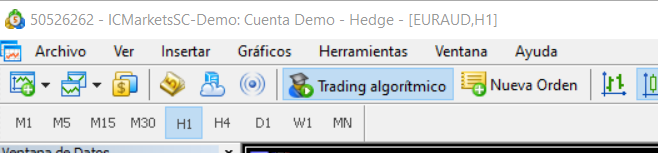
\includegraphics[width=1\textwidth]{imagenes/boton_trading_algoritmico.png}
	\caption{Opción a habilitar para mandar órdenes de operaciones al terminal MT5.} \label{boton_trading_algoritmico}
\end{figure}

Nota: para comprar y vender, he creado cuentas demo en el bróker de ICMarkets. Más información sobre brokers en el punto 2 de la memoria. \newline

El PR que completa este desarrollo es el \href{https://github.com/mcarmona99/TFG/pull/19}{\#19}. \newline

Para realizar las compras y ventas desde nuestro script, tenemos que hacer uso de la función \textit{order\_send}, proporcionada por la librería \textit{MetaTrader}.

\begin{figure}[h]
	\begin{lstlisting}[language=Python]
order_send(
	request      # estructura de la solicitud
);
	\end{lstlisting}
\end{figure}


\textit{request} es una estructura del tipo \textit{MqlTradeRequest} que describe la acción comercial necesaria. Parámetro no nombrado obligatorio.  \newline

Un ejemplo de request ya parametrizado podría ser el siguiente:\newline

\begin{figure}[h]
	\begin{lstlisting}[language=Python]
request = {
	"action": mt5.TRADE_ACTION_DEAL,
	"symbol": symbol,
	"volume": lot if lot else 0.01,
	"type": mt5.ORDER_TYPE_BUY if action.lower() == "buy" else mt5.ORDER_TYPE_SELL,
	"price": price,
	"sl": stop_lose,
	"tp": take_profit,
	"deviation": deviation,
	"magic": 234000,
	"comment": "python script open",
	"type_time": mt5.ORDER_TIME_GTC,
	"type_filling": mt5.ORDER_FILLING_IOC,
}

order_result = mt5.order_send(request)
	\end{lstlisting}
\end{figure}

Como vemos, se utiliza la opción \textit{mt5.ORDER\_TYPE\_BUY} para ordenar compras y \textit{mt5.ORDER\_TYPE\_SELL} para ventas.

Al intentar usar esta función sin tener el botón anteriormente mencionado habilitado, obtendremos la siguiente respuesta:\newline

\begin{figure}[h]
	\begin{lstlisting}
OrderSendResult(retcode=10027, deal=0, order=0, volume=0.0, price=0.0, bid=0.0, ask=0.0, comment='AutoTrading disabled by client', request_id=0, retcode_external=0, request=TradeRequest(action=1, magic=234000, order=0, symbol='EURUSD', volume=0.01, price=1.19432, stoplimit=0.0, sl=1.1933200000000002, tp=1.19532, deviation=20, type=0, type_filling=2, type_time=0, expiration=0, comment='python script open', position=0, position_by=0))
	\end{lstlisting}
\end{figure}

Tras probar con el método de Wyckoff, conseguimos una operativa en tiempo real que funciona correctamente, realizamos compras y ventas según criterios en tiempo real.

\subsection{Sprint 6: 30 agosto - 6 septiembre. Desarrollo de la gestión de datos y últimas correcciones}

En este último sprint se realizan las últimas tareas del proyecto. Entre ellas, la gestión de datos que hasta ahora se hacía en local y algunas correcciones menores y mejoras de diseño. \newline

\subsubsection{Issue 20: Última iteración del proyecto.}

Esta issue realizar los últimos desarrollos y correcciones del trabajo.\newline

En este punto se actualiza el estilo de la interfaz de la aplicación. Se añade un logo y colores para realizar una mejora en su diseño. \newline

Se añade aquí el sistema de gestión de datos. Cada usuario podrá seleccionar mercado, fecha de inicio de datos históricos y marco de tiempo en el que se guardarán en el formato \textit{OHLC}. Estos datos se guardarán en la sesión del usuario, en un nuevo campo que será \textit{TextField} y tendrá guardados los datos en formato \textit{csv}. Esta variable o campo del modelo \textit{Sesion} será accedido por cada una de las funciones de la APP tales como visualización de datos o backtesting para hacer uso de los datos. \newline

Se ha hecho también una actualización en la visualización de los datos antiguos para adaptar la funcionalidad a lo comentado en el párrafo anterior.\newline

La funcionalidad de backtesting ha sido actualizada también. Ahora, existe la posibilidad de realizar backtesting con marco de tiempo. Antes esto estaba fijado al marco \textit{H1}.\newline

Por último, en esta issue se mejora la salida de las gráficas de backtesting. Ahora tenemos más verbose en las gráficas y han sido formateadas.\newline

Se añaden también las decisiones tomadas por el algoritmo en el modo de trading en tiempo real y backtesting.\newline




\section{Diseño final de la interfaz}

En esta última sección de la implementación, añado el diseño final de la interfaz de la aplicación web.

\subsection{Página principal y formulario de Login}

Diseño en la figura \ref{1}

\begin{figure}[h]
	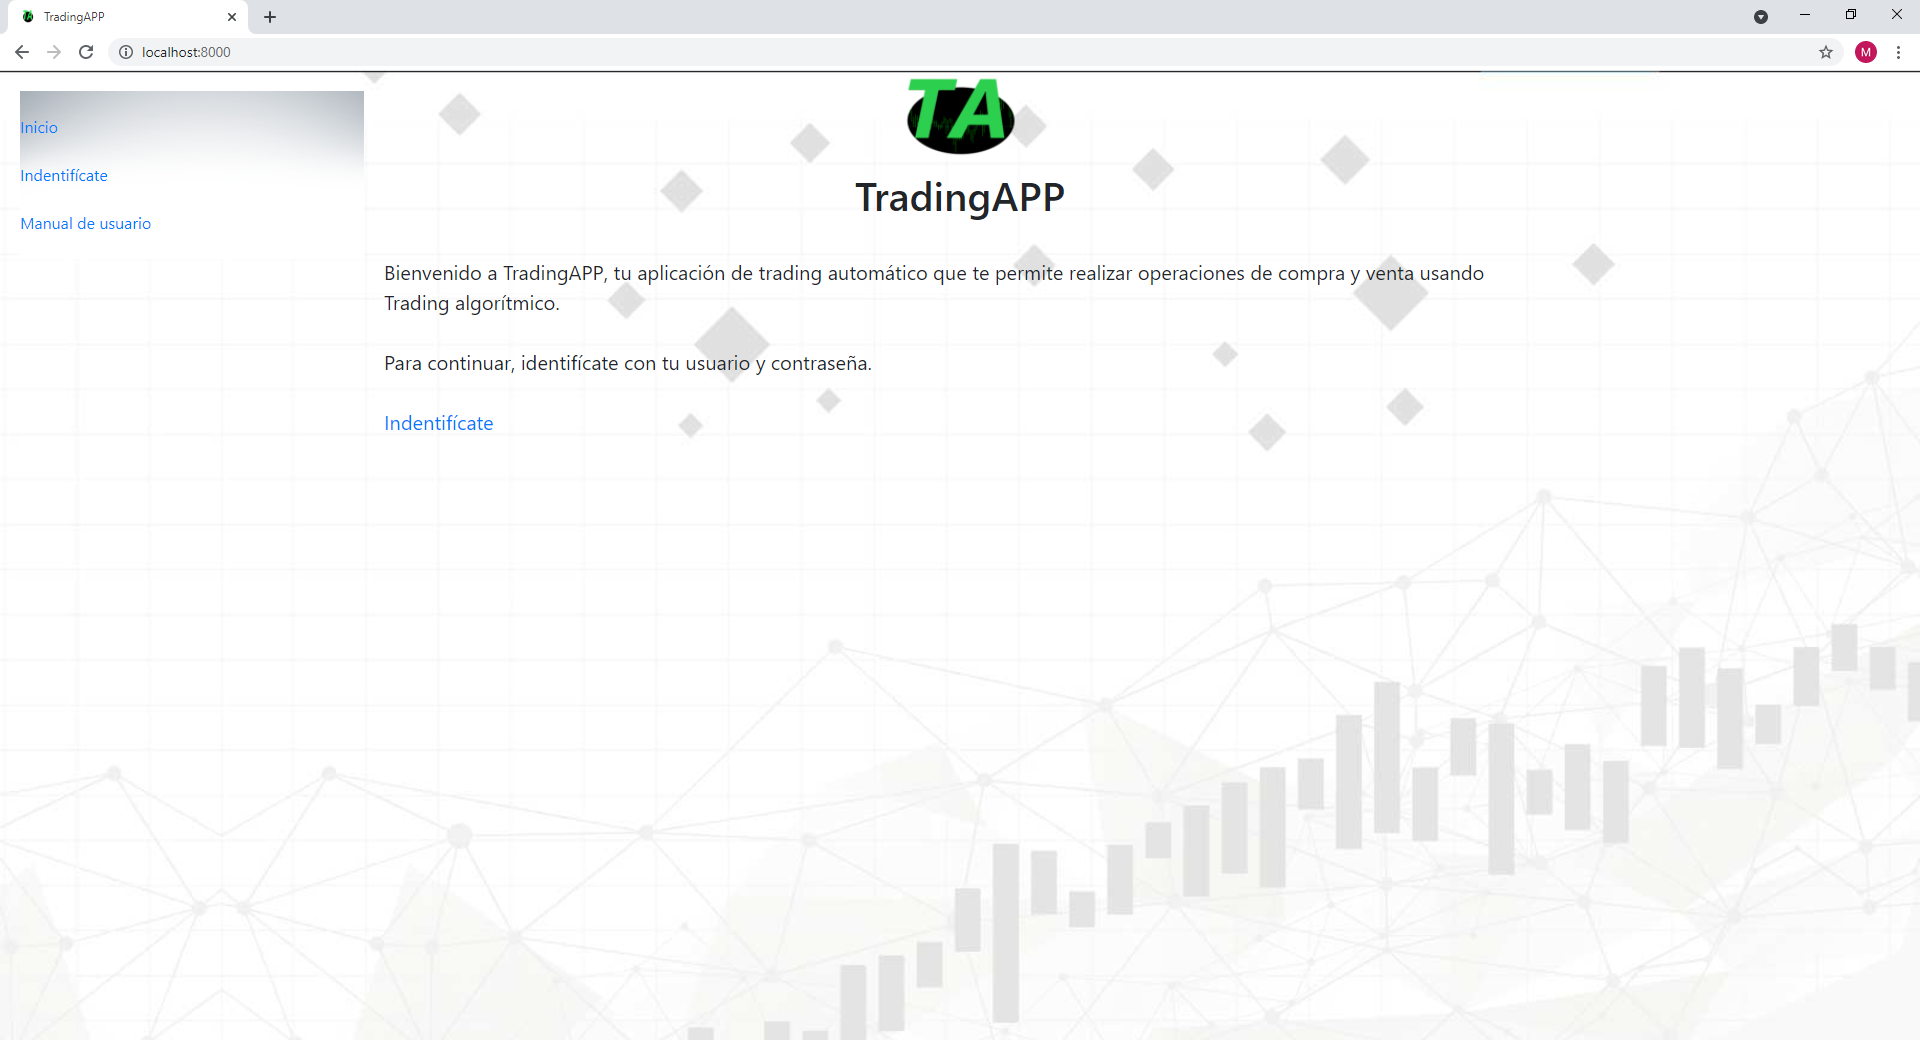
\includegraphics[width=1.2\textwidth]{imagenes/diseno_final/pagina_principal.png}\newline \\
	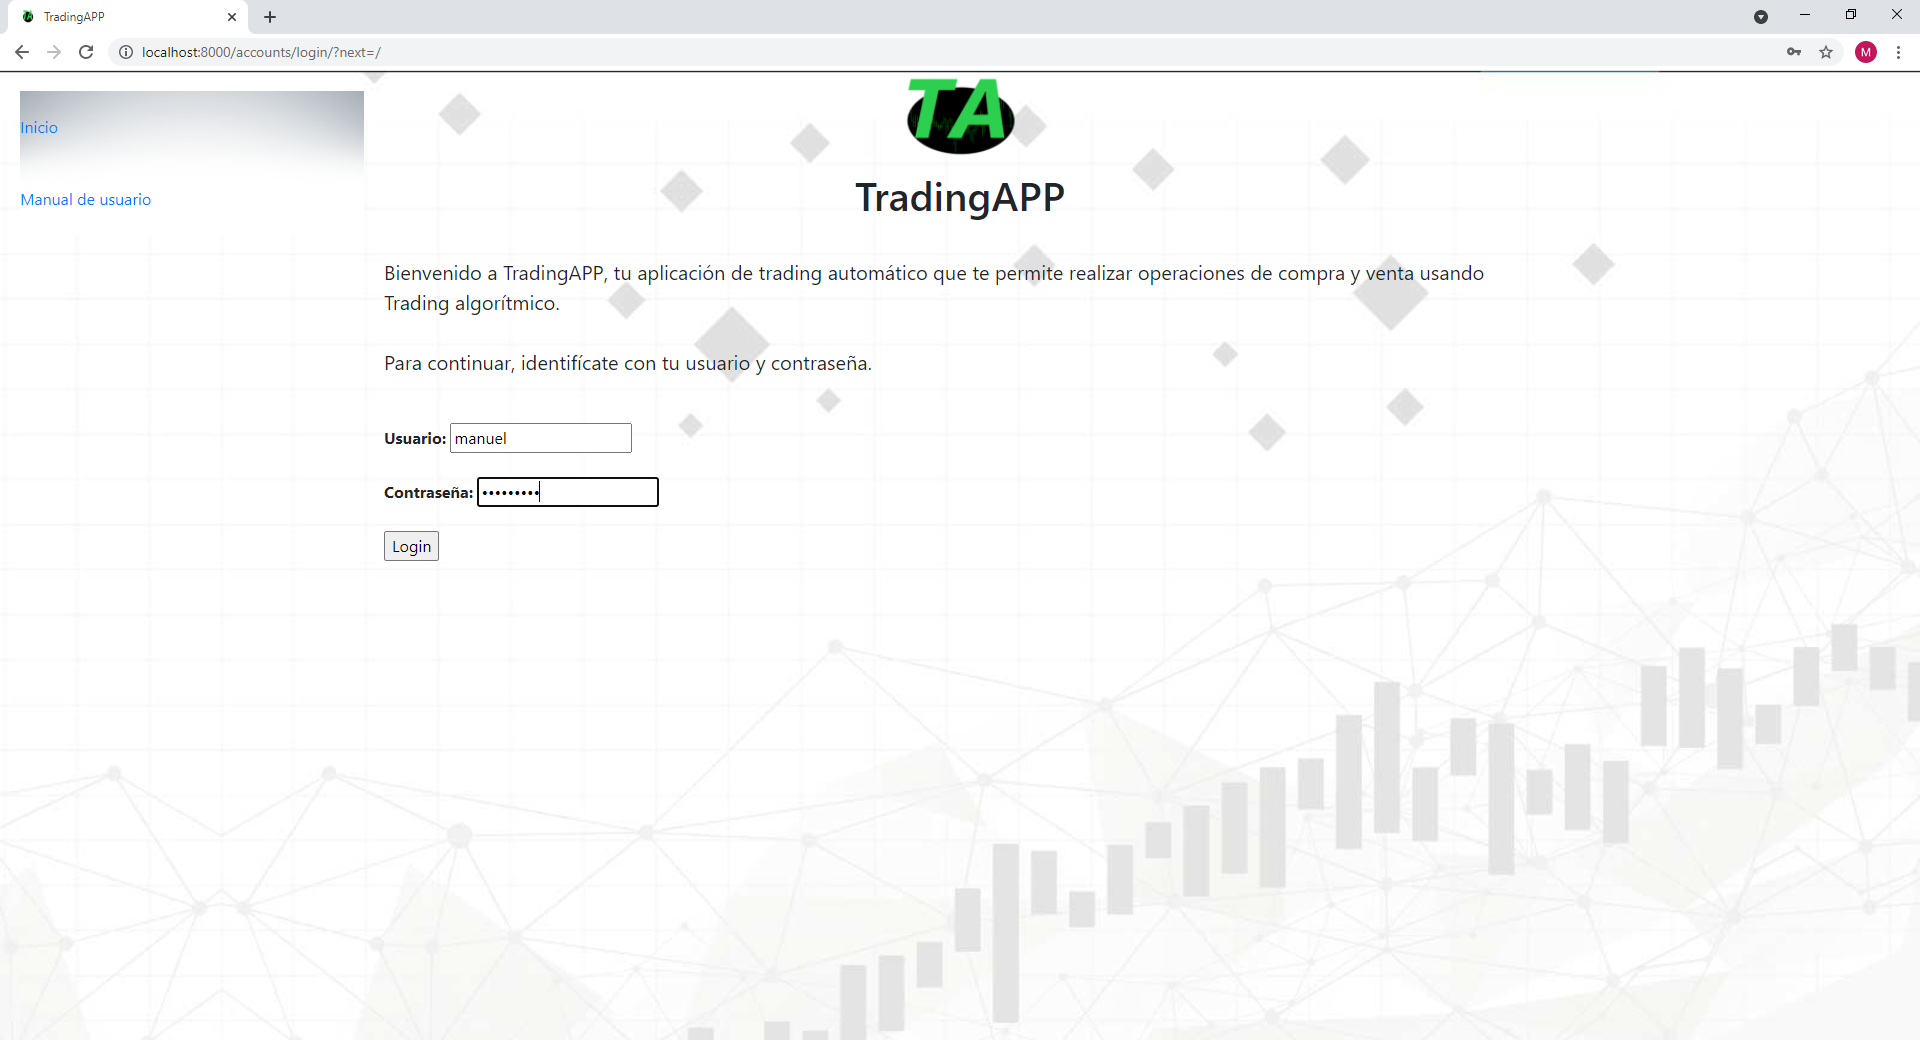
\includegraphics[width=1.2\textwidth]{imagenes/diseno_final/login.png}
	
	\caption{Página principal y formulario de login, respectivamente.} \label{1}
\end{figure}

\subsection{Menú principal y manual de usuario}
Diseño en la figura \ref{2}

\begin{figure}[h]
	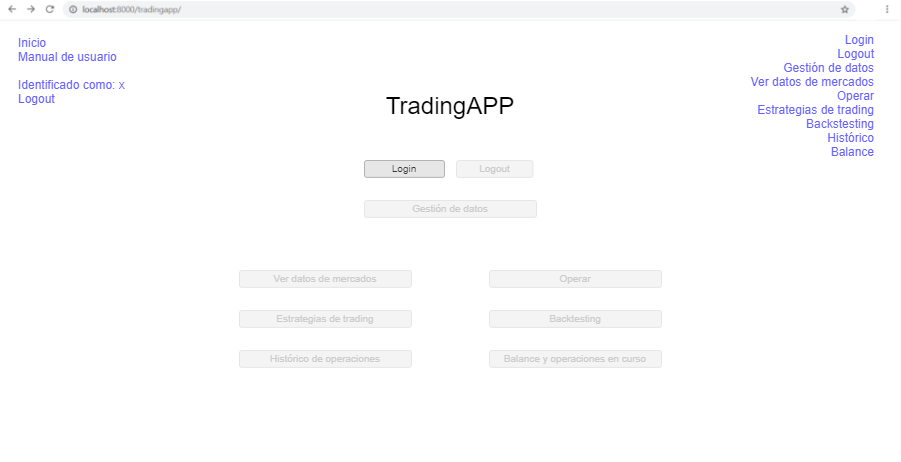
\includegraphics[width=1.2\textwidth]{imagenes/diseno_final/menu_principal.png}\newline \\
	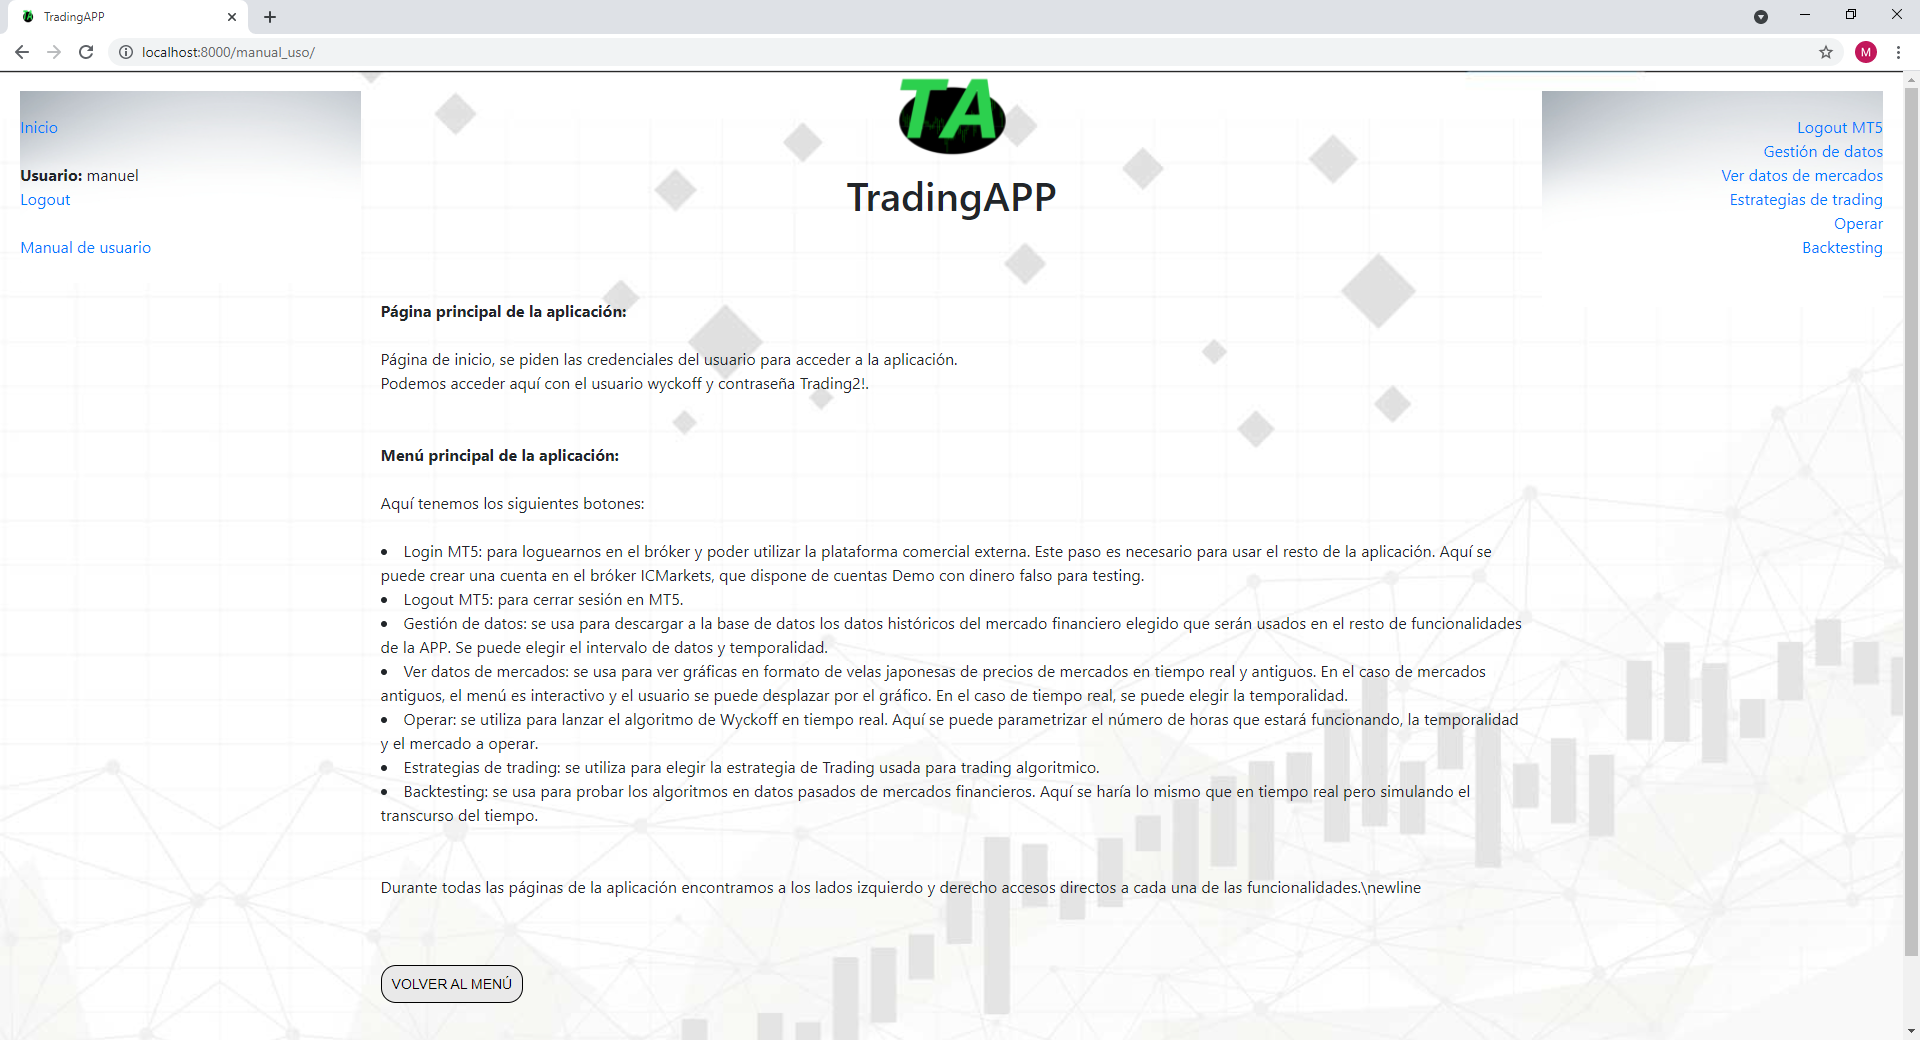
\includegraphics[width=1.2\textwidth]{imagenes/diseno_final/manual_usuario.png}

	\caption{Página principal y manual de usuario, respectivamente.}  \label{2}
\end{figure}

\subsection{Menús de elección de estrategia}
Diseño en la figura \ref{3}

\begin{figure}[h]
	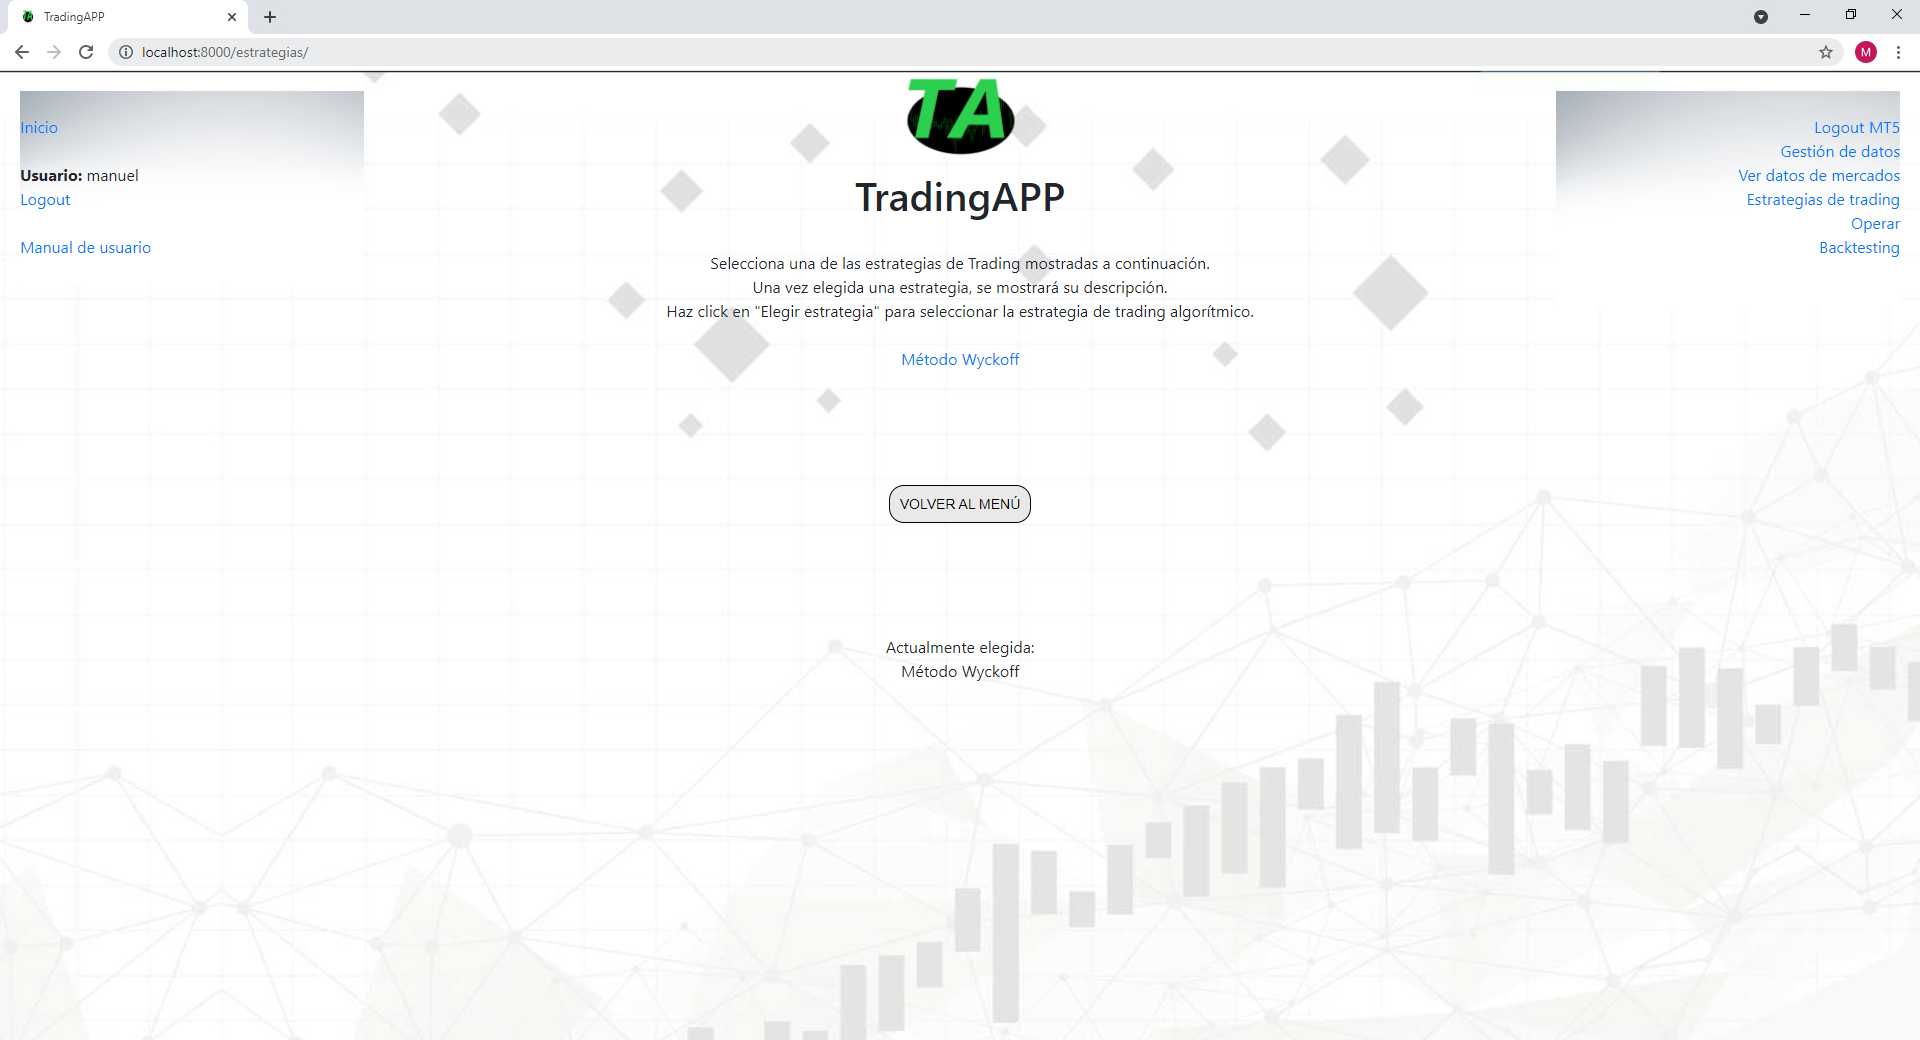
\includegraphics[width=1.2\textwidth]{imagenes/diseno_final/menu_eleccion_estrategia.png}\newline \\
	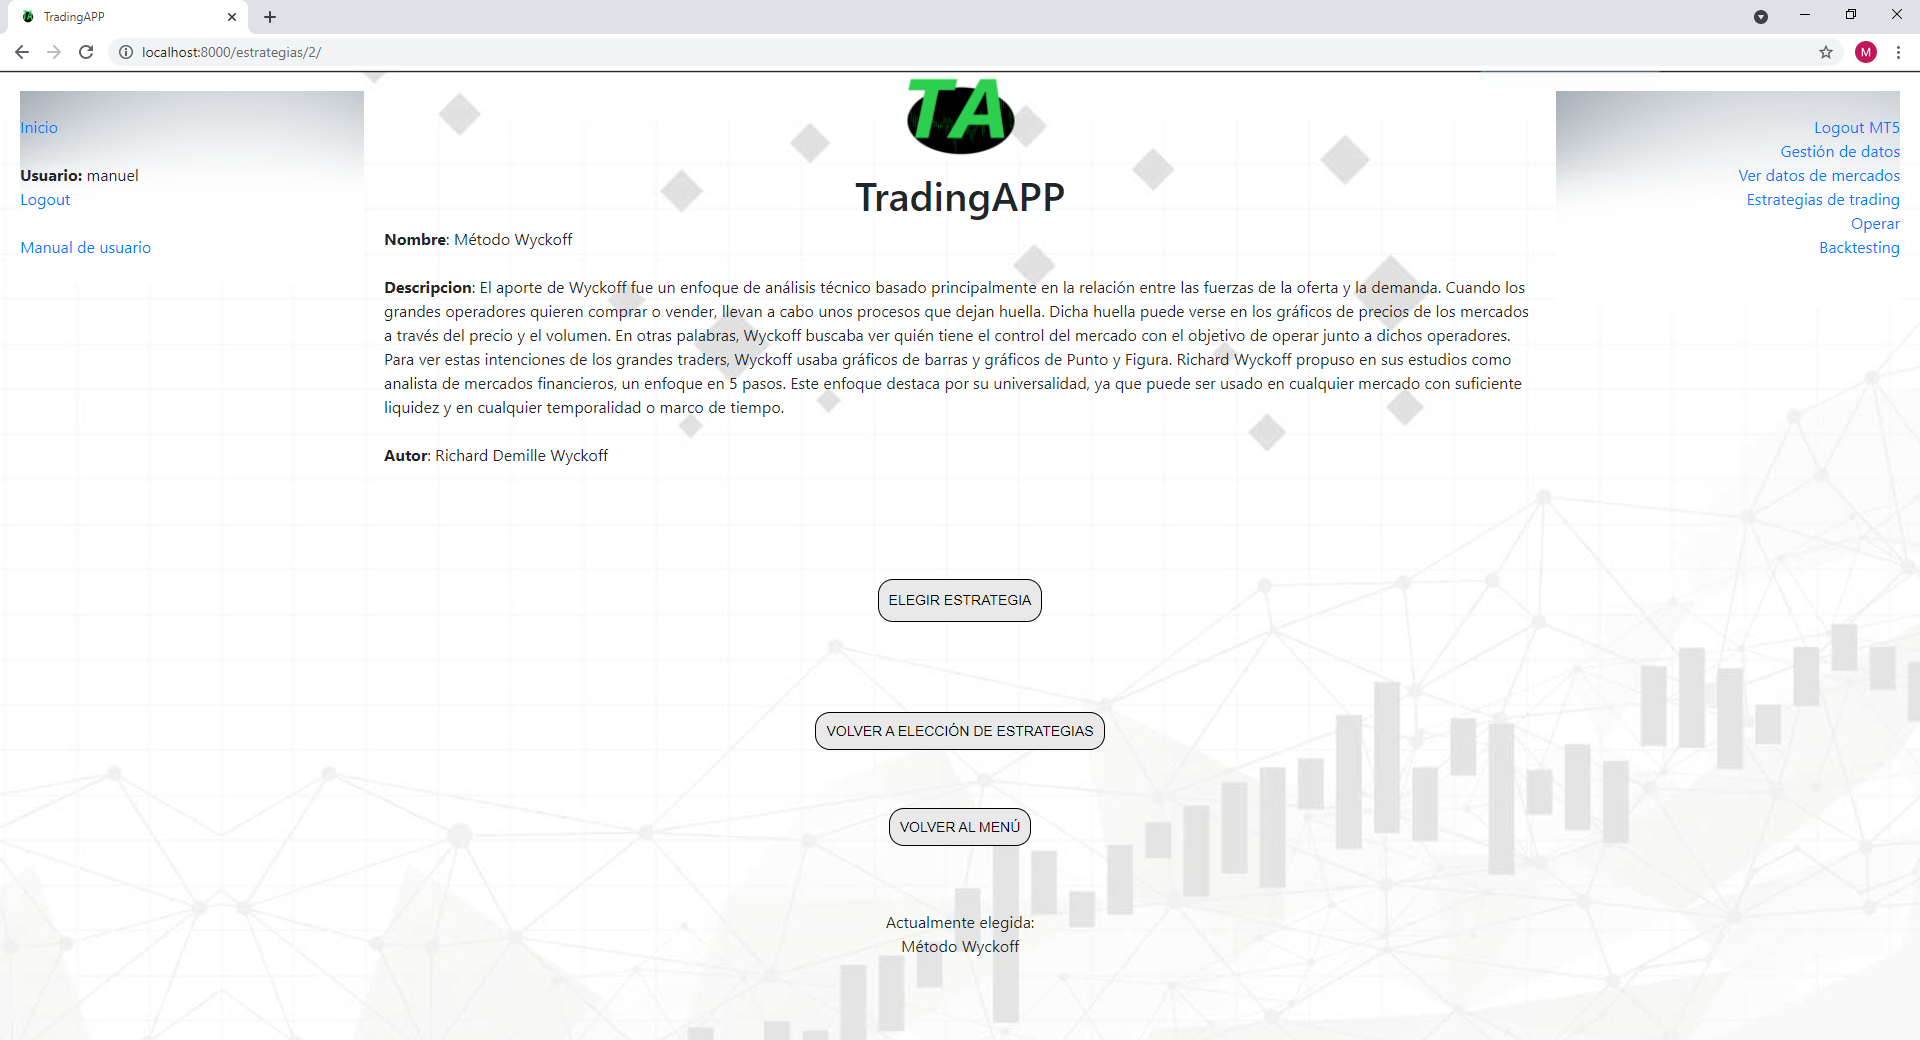
\includegraphics[width=1.2\textwidth]{imagenes/diseno_final/menu_eleccion_estrategia_2.png}
	
	\caption{Menús de elección de estrategia.}  \label{3}
\end{figure}

\subsection{Menú de backtesting y operativa en tiempo real}
Diseño en la figura \ref{4}

\begin{figure}[h]
	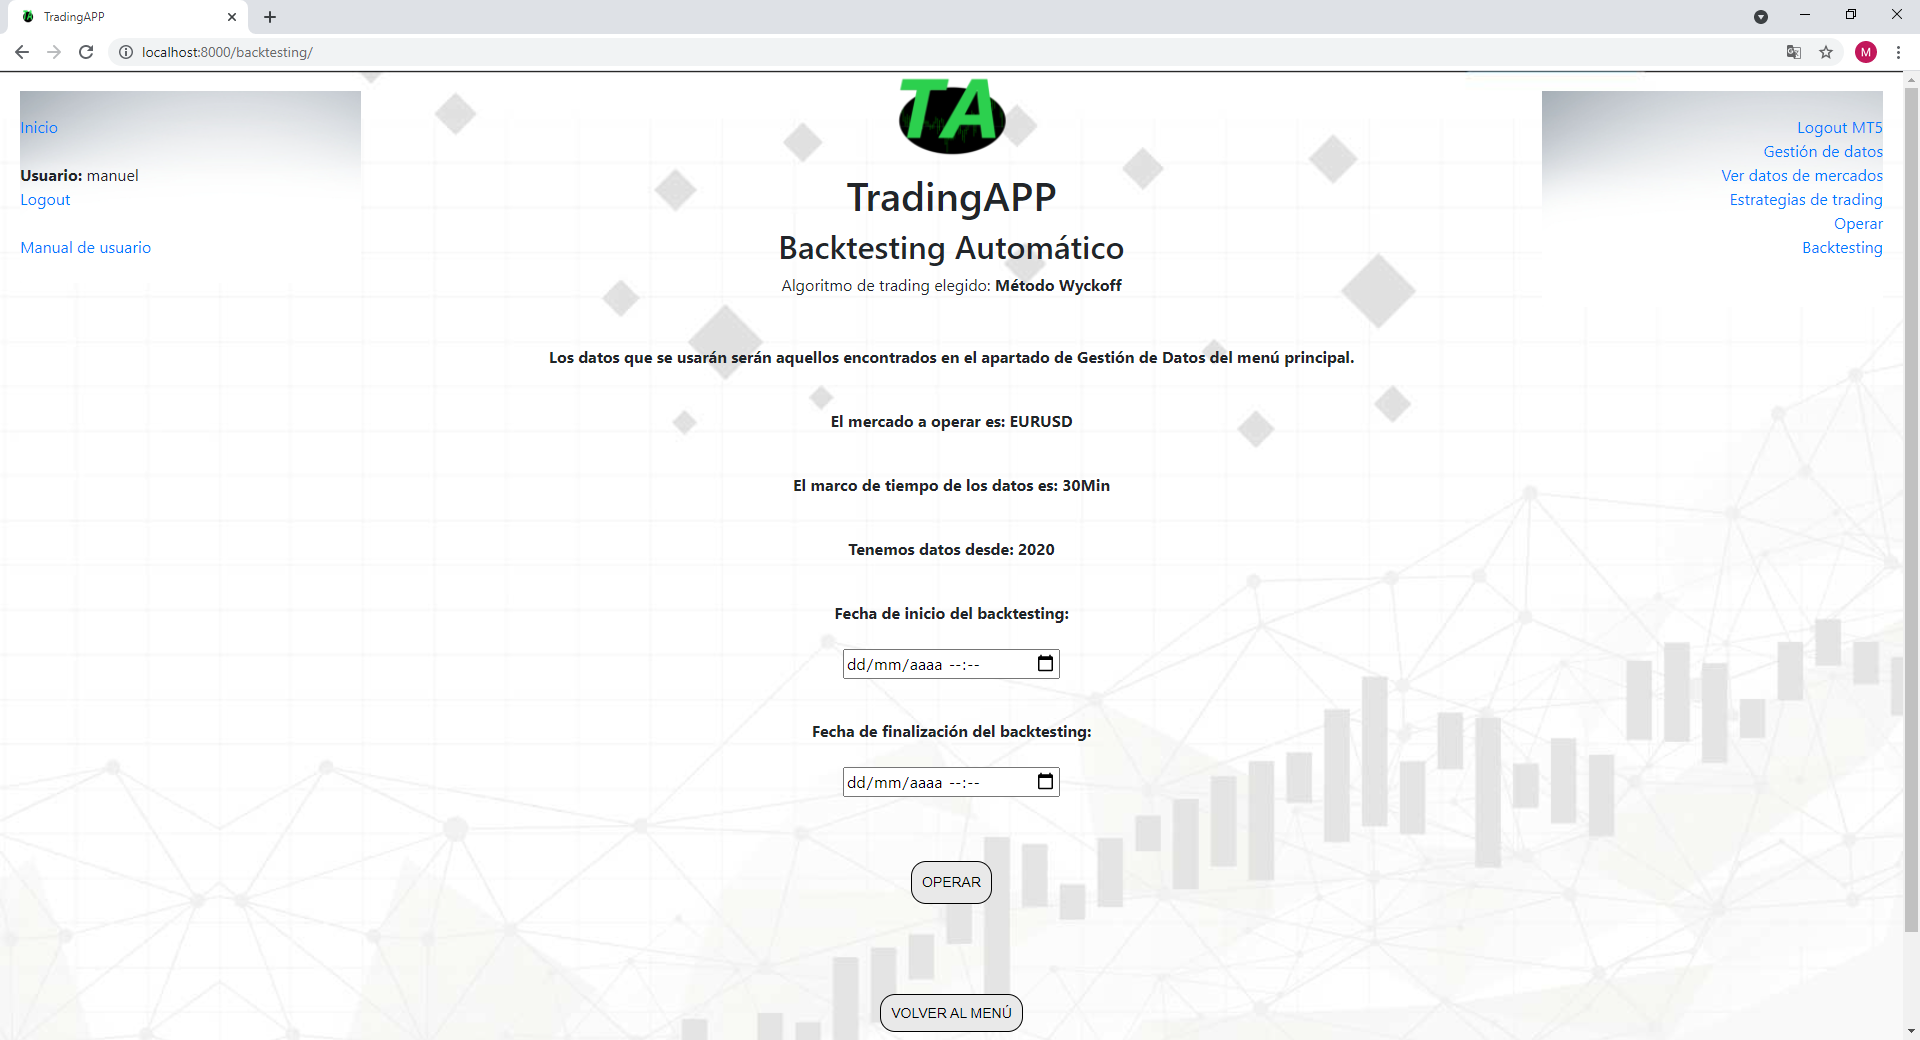
\includegraphics[width=1.2\textwidth]{imagenes/diseno_final/menu_backtesting.png}\newline \\
	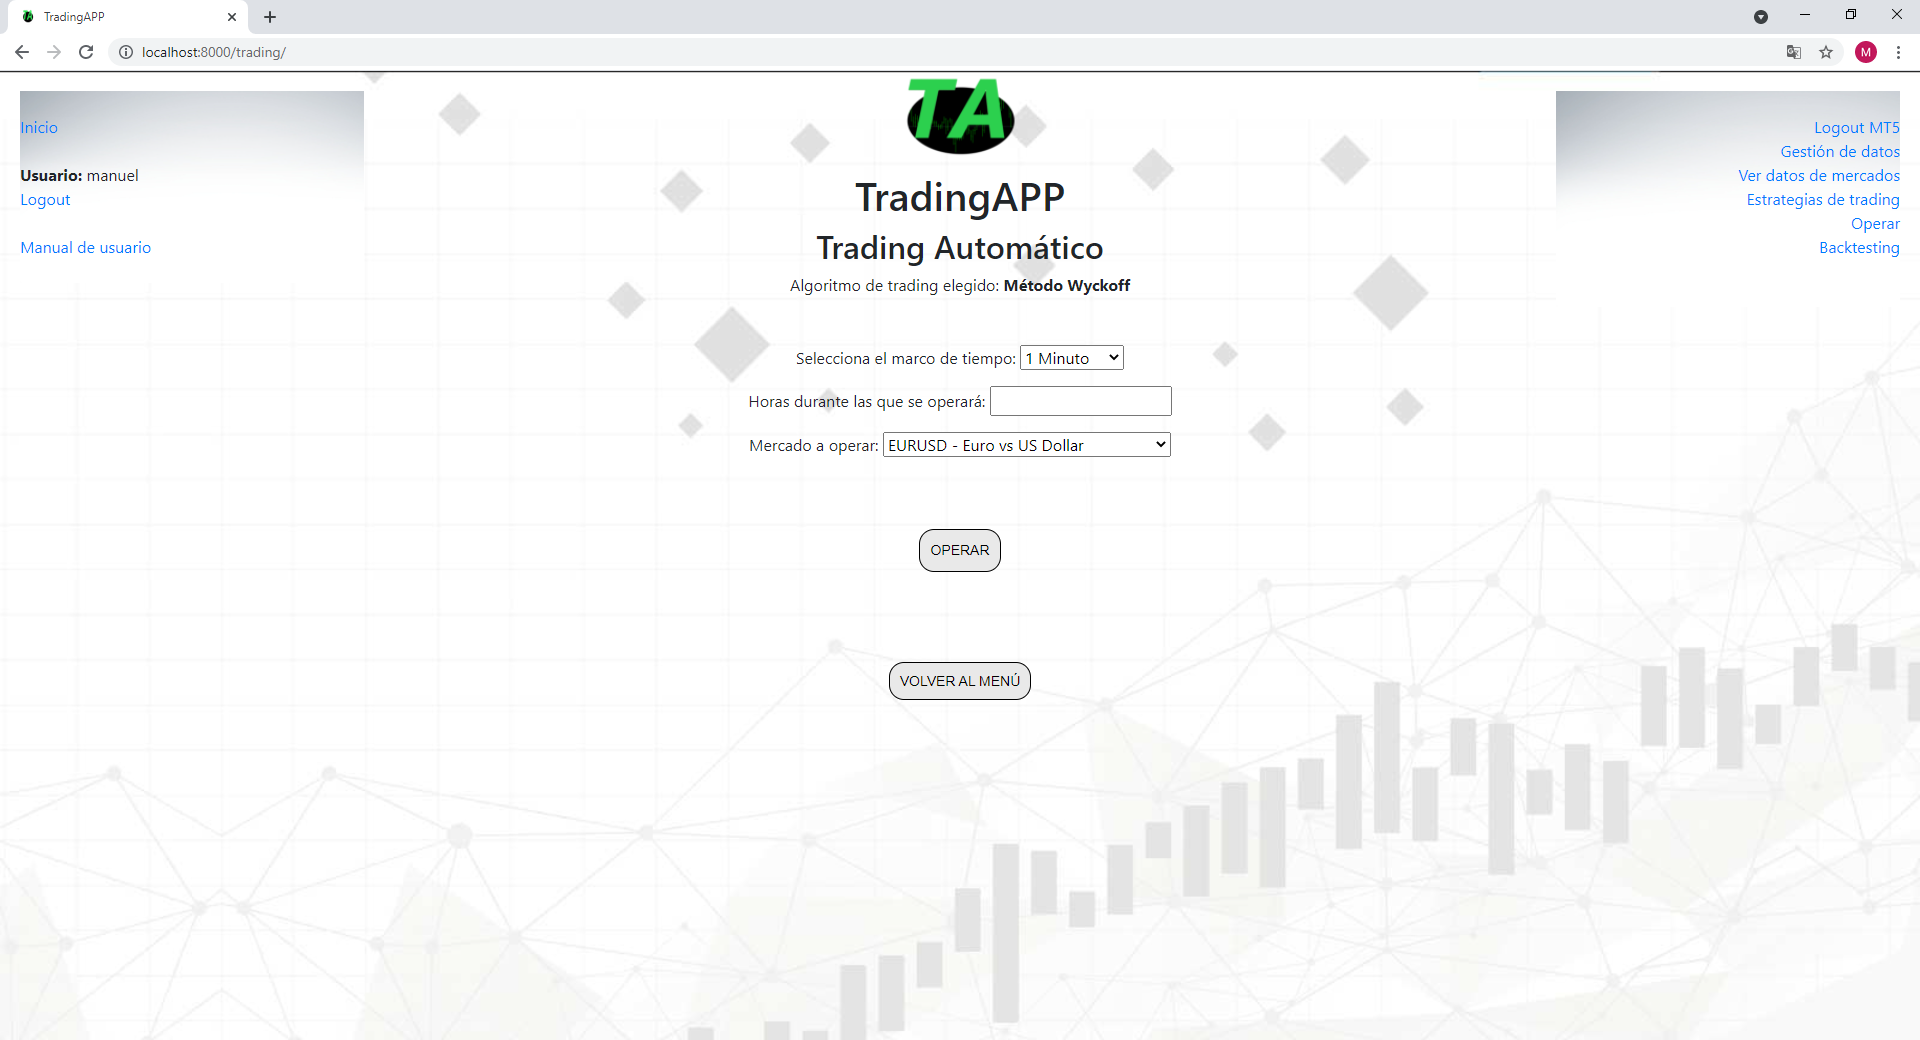
\includegraphics[width=1.2\textwidth]{imagenes/diseno_final/menu_trading_tiempo_real.png}
	
	\caption{Menú de backtesting y trading a tiempo real, respectivamente.}  \label{4}
\end{figure}

\subsection{Menú de gestión de datos}
Diseño en la figura \ref{5}

\begin{figure}[h]
	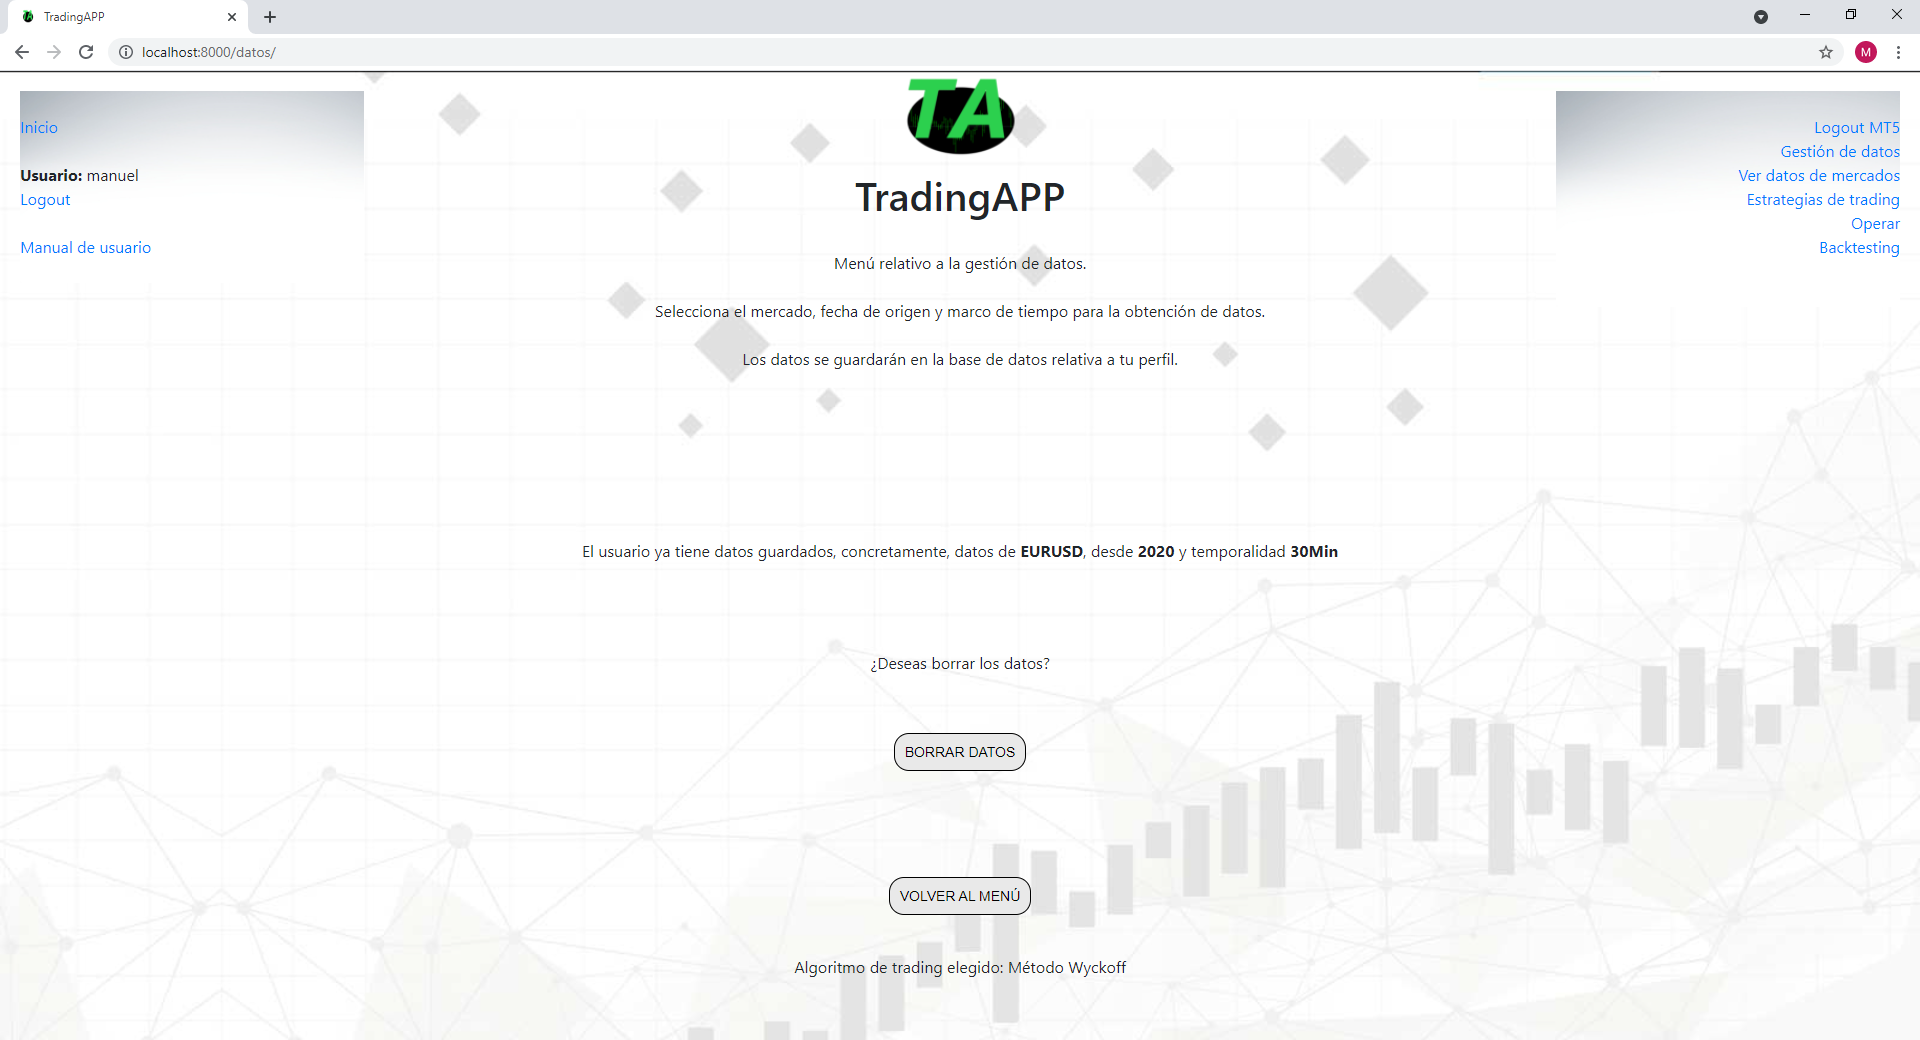
\includegraphics[width=1.2\textwidth]{imagenes/diseno_final/menu_gestion_datos.png}\newline \\
	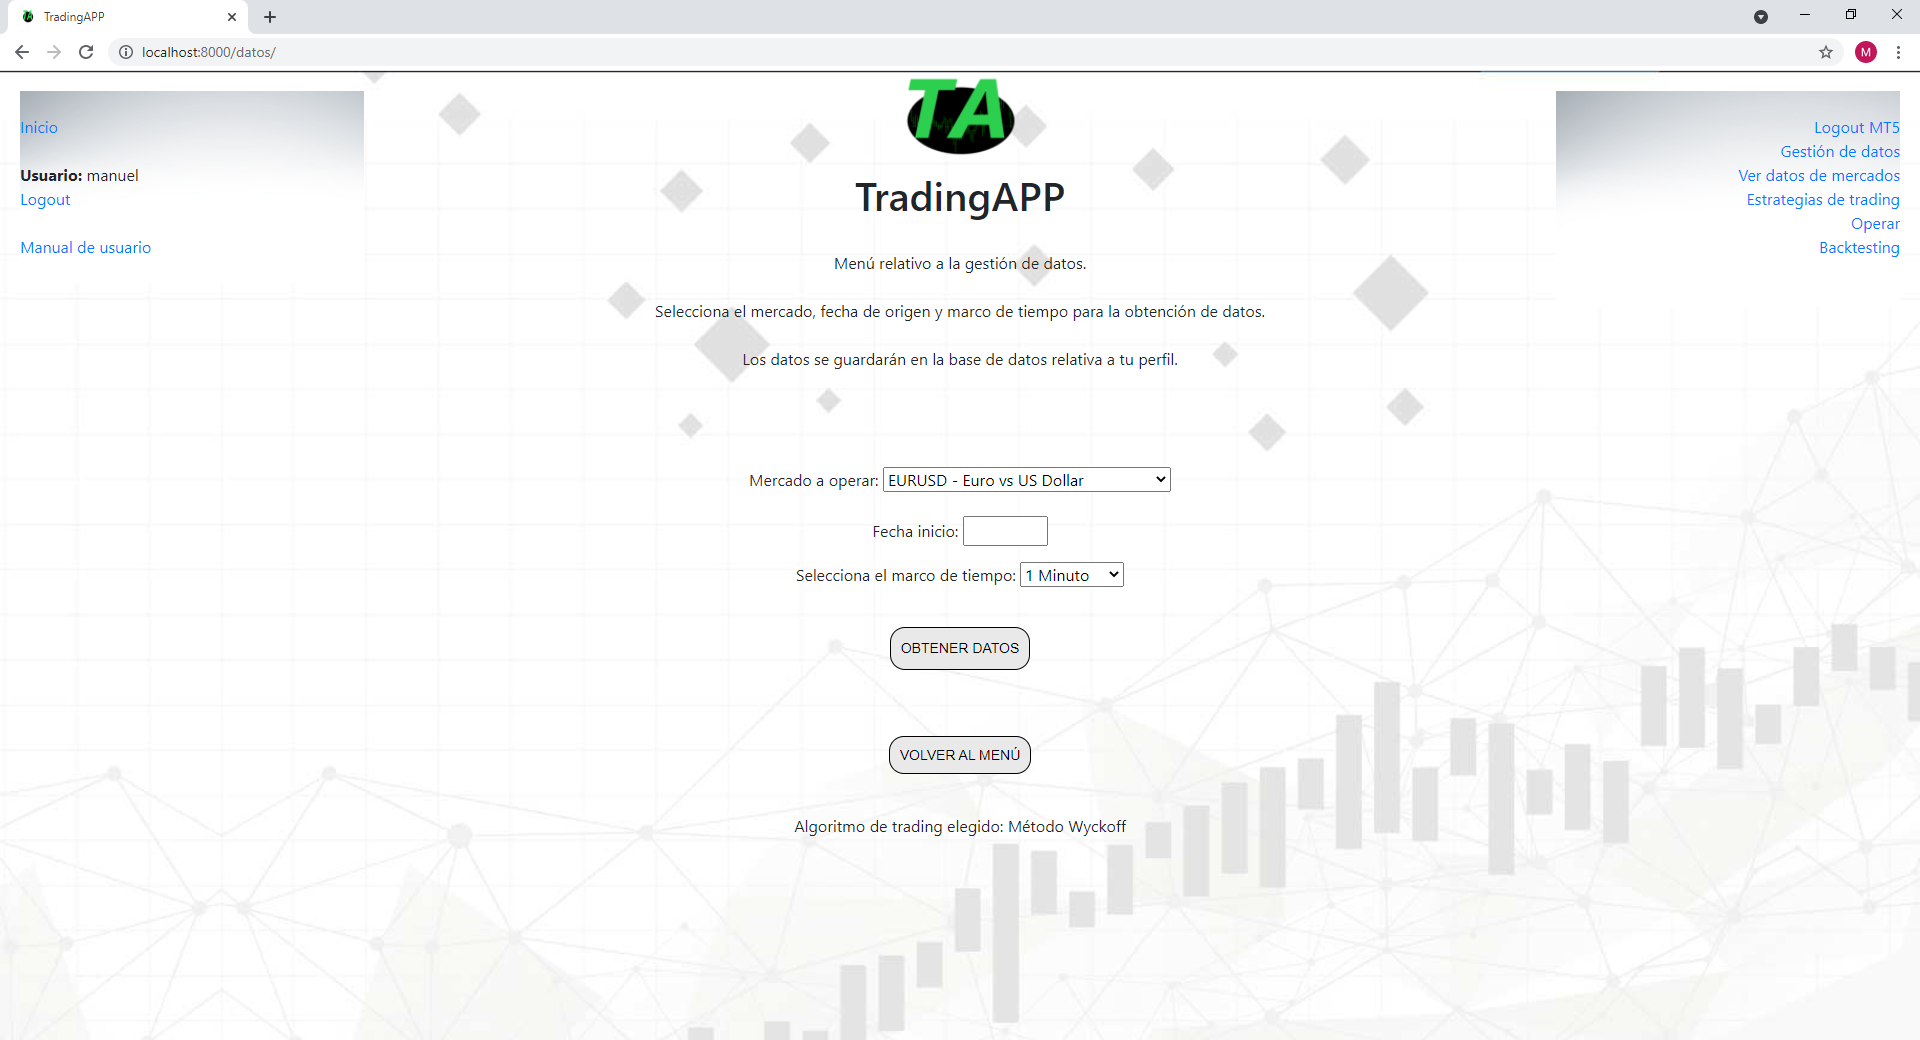
\includegraphics[width=1.2\textwidth]{imagenes/diseno_final/menu_gestion_datos_borrados.png}
	
	\caption{Menús de gestión de datos, teniendo datos guardados y sin tenerlos, respectivamente.}  \label{5}
\end{figure}

\subsection{Menú de visualización de datos}
Diseños en las figuras \ref{6} y \ref{7}.

\begin{figure}[h]
	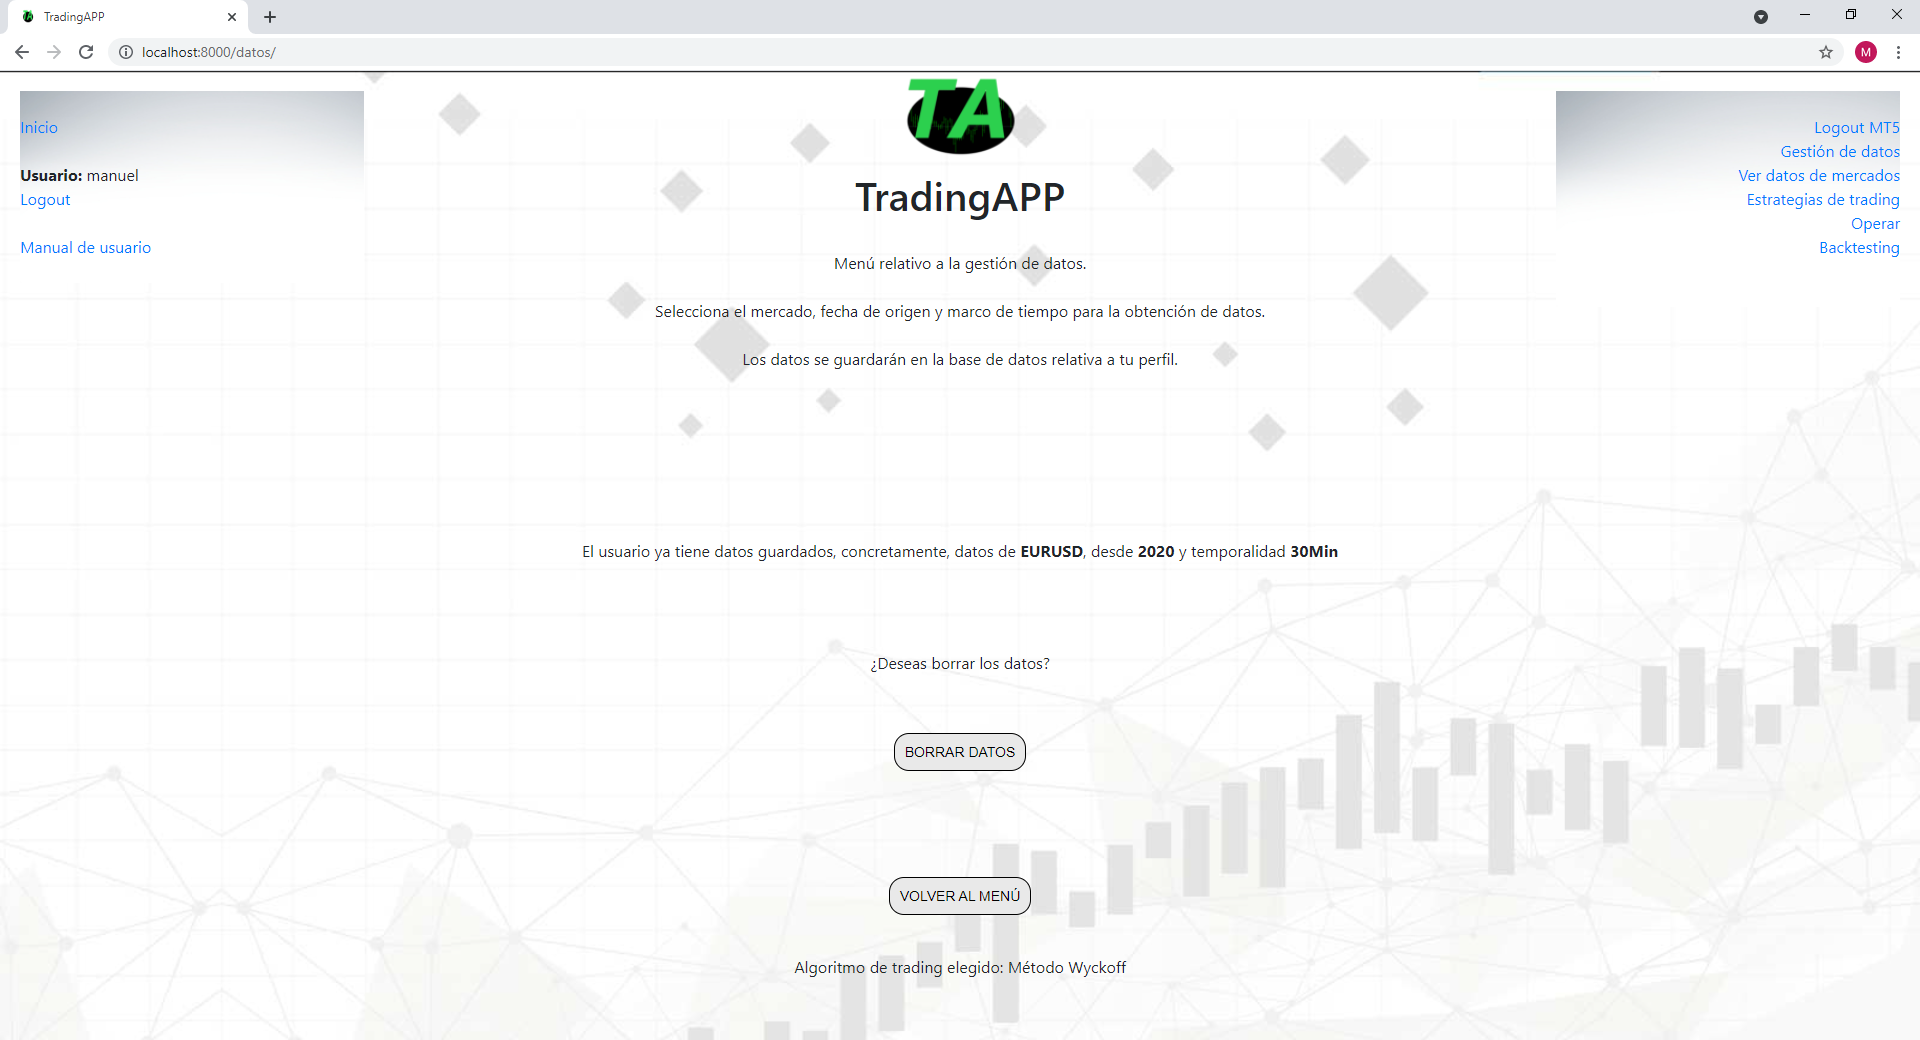
\includegraphics[width=1.2\textwidth]{imagenes/diseno_final/menu_visualizacion_datos.png}\newline \\
	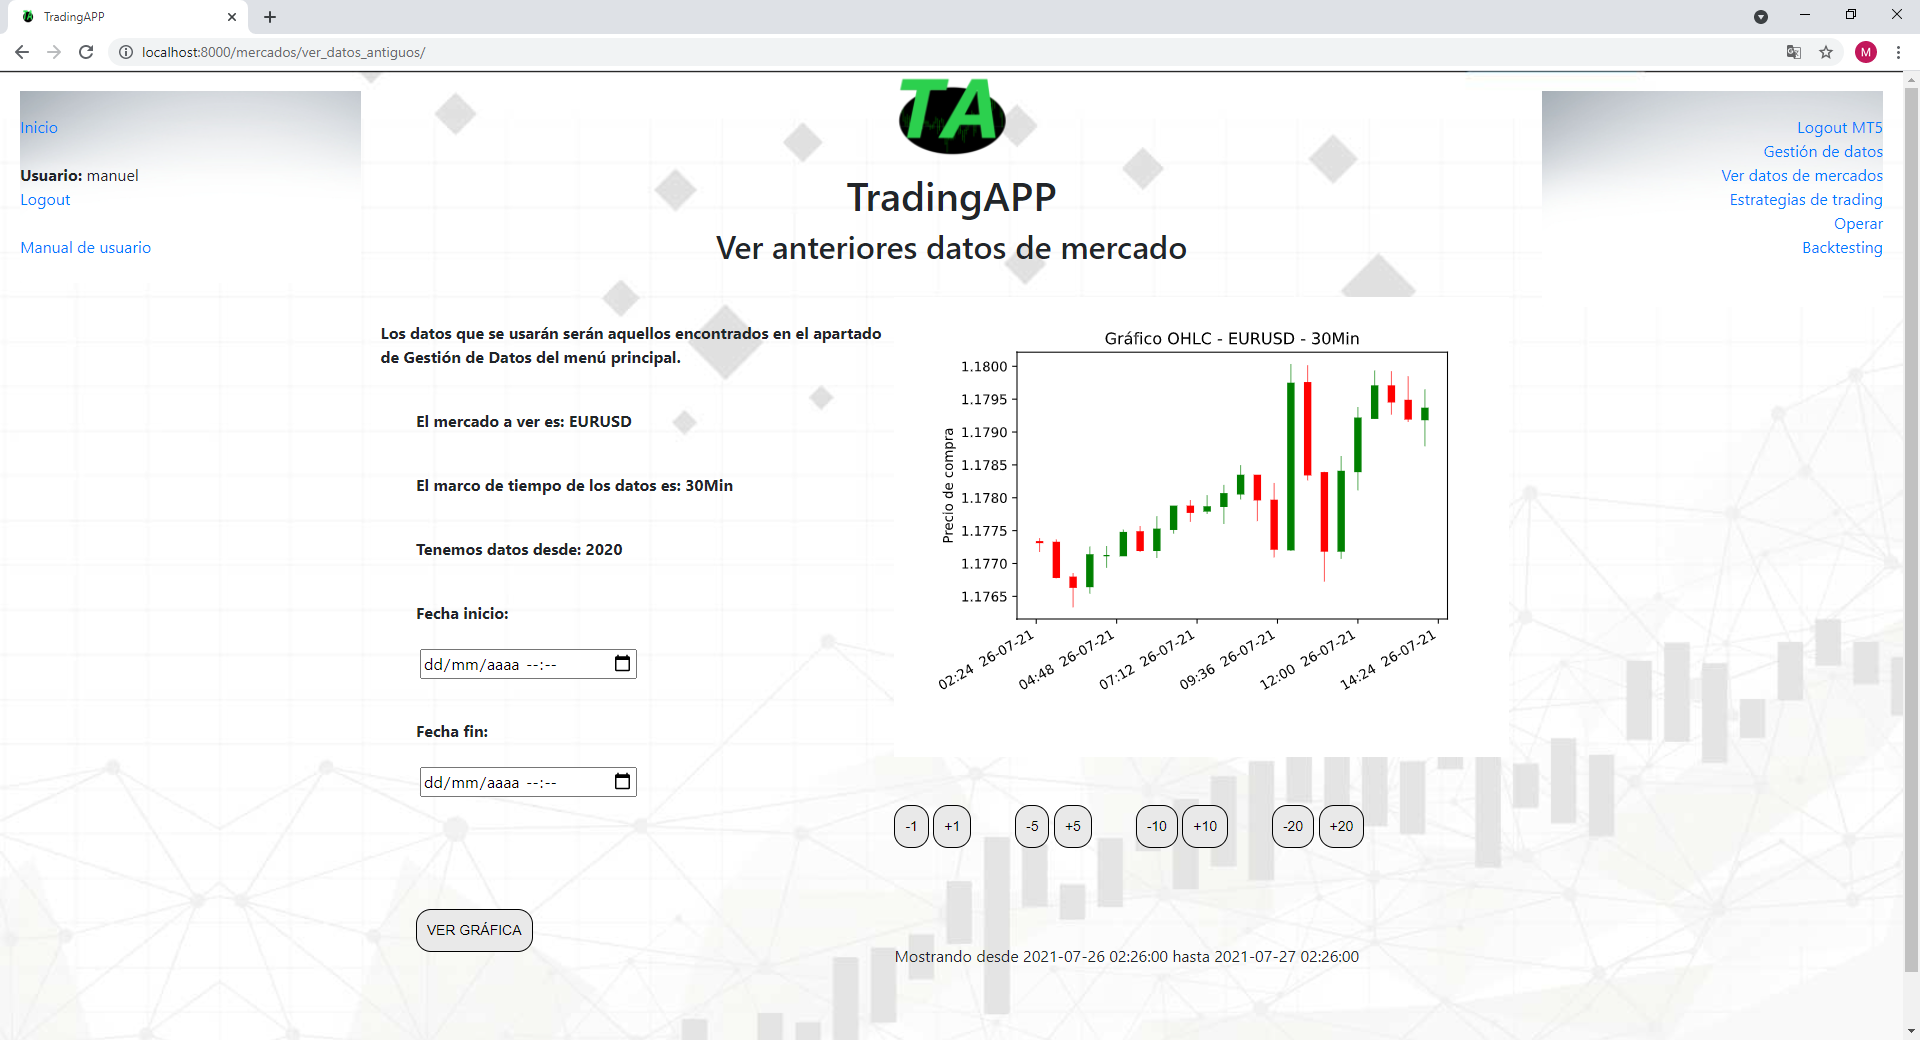
\includegraphics[width=1.2\textwidth]{imagenes/diseno_final/menu_visualizacion_datos_antiguos.png}
	
	\caption{Menús de visualización de datos antiguos.}  \label{6}
\end{figure}

\begin{figure}[h]
	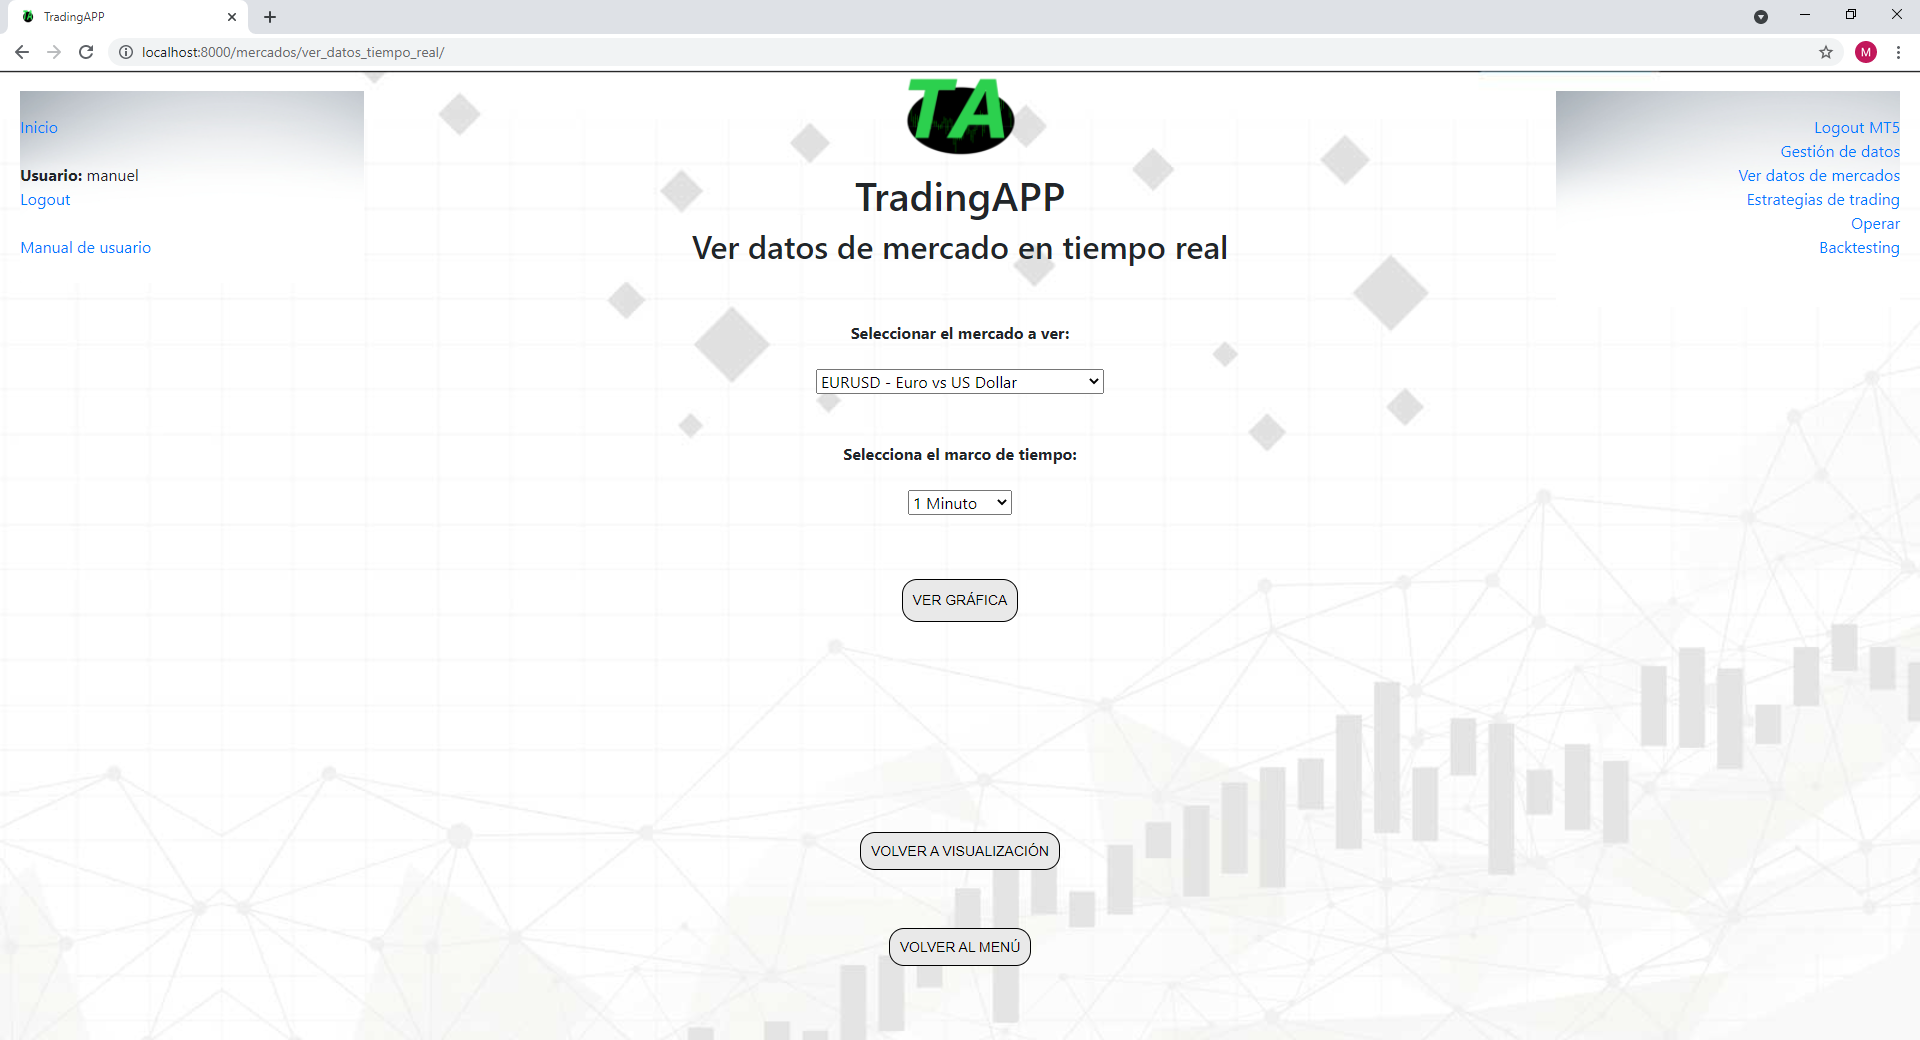
\includegraphics[width=1.2\textwidth]{imagenes/diseno_final/menu_visualizacion_datos_tpo_real.png}
	
	\caption{Menú de visualización de datos en tiempo real.}  \label{7}
\end{figure}


	